         \chapter{Magnetism}\fancyfoot[LO,RE]{Physics: Electricity and Magnetism}
    \setcounter{figure}{1}
    \setcounter{subfigure}{1}
    \label{m37830}
    \section{Introduction}
%            \label{m37830*cid2} $ \hspace{-5pt}\begin{array}{cccccccccccc}   \end{array} $ \hspace{2 pt}\raisebox{-0.2em}{
\includegraphics[height=1em]{../icons/www.eps}} {(section shortcode: P10064 )} \par 

\begin{minipage}{.5\textwidth}
      \label{m37830*id127925}Magnetism is a force that certain kinds of objects, which are called `magnetic' objects, can exert on each other without physically touching. A magnetic object is surrounded by a magnetic `field' that gets weaker as one moves further away from the object. A second object can feel a magnetic force from the first object because it feels the magnetic field of the first object.\par 
      \label{m37830*id127932}Humans have known about magnetism for many thousands of years.
For example, \textsl{lodestone} is a magnetised form of the iron oxide mineral
\textsl{magnetite}. It has the property of attracting iron
objects. It is referred to in old European and Asian historical
records; from around 800 \textsc{BCE} in Europe and around
2~600 \textsc{BCE} in Asia.\par
\end{minipage}
\begin{minipage}{.5\textwidth}
\begin{center}
\textbf{Magnetic objects stuck to a magnet}\par
 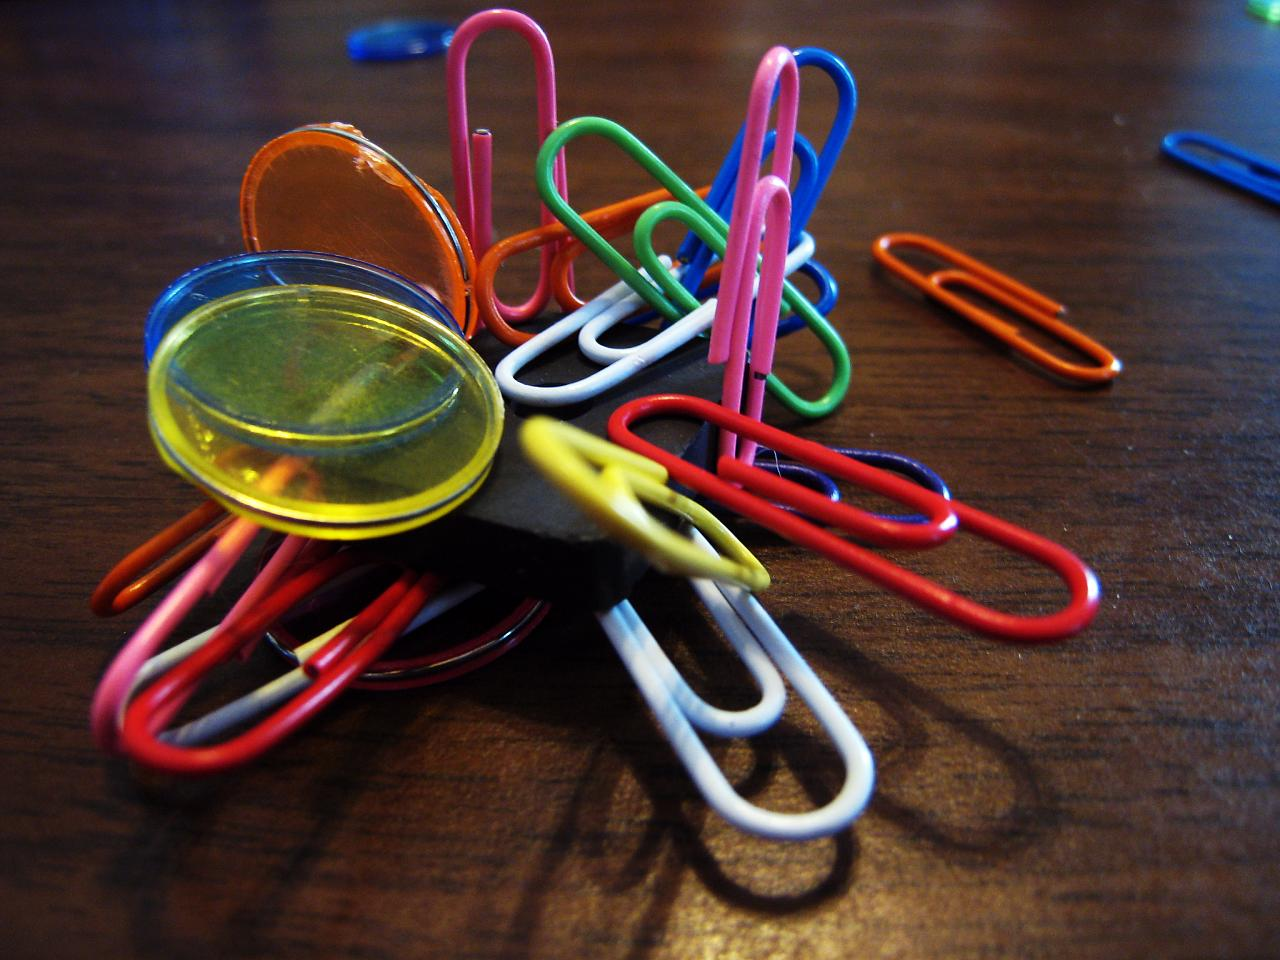
\includegraphics[width=.8\textwidth]{photos/magnet_mess_dougww.jpg}\par
\textit{Photograph by dougww on Flickr}
\end{center}
\end{minipage}
 
\IFact{The root of the English word \textsl{magnet} is from the Greek word \textsl{magnes}, probably from Magnesia in Asia Minor, once an important source of lodestone.}

    \section*{Magnetic fields}
%            \label{m37830*cid3} $ \hspace{-5pt}\begin{array}{cccccccccccc}   \end{array} $ \hspace{2 pt}\raisebox{-0.2em}{
\includegraphics[height=1em]{../icons/www.eps}} {(section shortcode: P10065 )} \par 
      \label{m37830*id128332}A magnetic field is a region in space where a magnet or object made of magnetic material will experience a non-contact force.\par 
      \label{m37830*id128337}Electrons inside any object have magnetic fields associated
with them. In most materials these fields point in all
directions, so the net magnetic field is zero. For example, in the plastic ball below,
the directions of the magnetic fields of the electrons (shown by the arrows) are pointing
in different directions and cancel each other out. Therefore the plastic ball is not magnetic and
has no magnetic field.\par 
      \label{m37830*id128346}
    \setcounter{subfigure}{0}
	\begin{figure}[H] % horizontal\label{m37830*id128349}
    \begin{center}
  \begin{pspicture}(0,-1.5089062)(11.060625,1.4689063)
\pscircle[linewidth=0.04,dimen=outer](3.663125,0.45890626){1.01}
\psline[linewidth=0.04cm,arrowsize=0.05291667cm 2.0,arrowlength=1.4,arrowinset=0.4]{->}(4.013125,0.98890626)(4.173125,1.2489063)
\psline[linewidth=0.04cm,arrowsize=0.05291667cm 2.0,arrowlength=1.4,arrowinset=0.4]{->}(2.933125,0.12890625)(3.213125,0.04890625)
\psline[linewidth=0.04cm,arrowsize=0.05291667cm 2.0,arrowlength=1.4,arrowinset=0.4]{->}(3.693125,-0.45109376)(3.633125,-0.19109374)
\psline[linewidth=0.04cm,arrowsize=0.05291667cm 2.0,arrowlength=1.4,arrowinset=0.4]{->}(3.933125,-0.07109375)(3.753125,-0.27109376)
\psline[linewidth=0.04cm,arrowsize=0.05291667cm 2.0,arrowlength=1.4,arrowinset=0.4]{->}(3.793125,-0.27109376)(4.113125,-0.33109376)
\psline[linewidth=0.04cm,arrowsize=0.05291667cm 2.0,arrowlength=1.4,arrowinset=0.4]{->}(3.133125,0.9089062)(3.413125,0.82890624)
\psline[linewidth=0.04cm,arrowsize=0.05291667cm 2.0,arrowlength=1.4,arrowinset=0.4]{->}(4.053125,0.22890624)(4.333125,0.14890625)
\psline[linewidth=0.04cm,arrowsize=0.05291667cm 2.0,arrowlength=1.4,arrowinset=0.4]{->}(2.833125,0.22890624)(2.993125,0.48890626)
\psline[linewidth=0.04cm,arrowsize=0.05291667cm 2.0,arrowlength=1.4,arrowinset=0.4]{->}(2.973125,0.60890627)(3.253125,0.5289062)
\psline[linewidth=0.04cm,arrowsize=0.05291667cm 2.0,arrowlength=1.4,arrowinset=0.4]{->}(2.833125,0.22890624)(2.993125,0.48890626)
\psline[linewidth=0.04cm,arrowsize=0.05291667cm 2.0,arrowlength=1.4,arrowinset=0.4]{->}(2.913125,0.70890623)(3.073125,0.9689062)
\psline[linewidth=0.04cm,arrowsize=0.05291667cm 2.0,arrowlength=1.4,arrowinset=0.4]{->}(2.913125,0.70890623)(3.073125,0.9689062)
\psline[linewidth=0.04cm,arrowsize=0.05291667cm 2.0,arrowlength=1.4,arrowinset=0.4]{->}(3.233125,-0.17109375)(3.393125,0.08890625)
\psline[linewidth=0.04cm,arrowsize=0.05291667cm 2.0,arrowlength=1.4,arrowinset=0.4]{->}(3.293125,0.26890624)(3.453125,0.5289062)
\psline[linewidth=0.04cm,arrowsize=0.05291667cm 2.0,arrowlength=1.4,arrowinset=0.4]{->}(3.313125,1.0289062)(3.473125,1.2889062)
\psline[linewidth=0.04cm,arrowsize=0.05291667cm 2.0,arrowlength=1.4,arrowinset=0.4]{->}(3.313125,1.0289062)(3.473125,1.2889062)
\psline[linewidth=0.04cm,arrowsize=0.05291667cm 2.0,arrowlength=1.4,arrowinset=0.4]{->}(3.513125,0.82890624)(3.673125,1.0889063)
\psline[linewidth=0.04cm,arrowsize=0.05291667cm 2.0,arrowlength=1.4,arrowinset=0.4]{->}(4.213125,0.7889063)(4.373125,1.0489062)
\psline[linewidth=0.04cm,arrowsize=0.05291667cm 2.0,arrowlength=1.4,arrowinset=0.4]{->}(4.073125,-0.19109374)(4.233125,0.06890625)
\psline[linewidth=0.04cm,arrowsize=0.05291667cm 2.0,arrowlength=1.4,arrowinset=0.4]{->}(4.553125,0.30890626)(4.273125,0.42890626)
\psline[linewidth=0.04cm,arrowsize=0.05291667cm 2.0,arrowlength=1.4,arrowinset=0.4]{->}(3.973125,0.74890625)(3.693125,0.86890626)
\psline[linewidth=0.04cm,arrowsize=0.05291667cm 2.0,arrowlength=1.4,arrowinset=0.4]{->}(3.673125,0.02890625)(3.393125,0.14890625)
\psline[linewidth=0.04cm,arrowsize=0.05291667cm 2.0,arrowlength=1.4,arrowinset=0.4]{->}(3.513125,0.60890627)(3.233125,0.7289063)
\psline[linewidth=0.04cm,arrowsize=0.05291667cm 2.0,arrowlength=1.4,arrowinset=0.4]{->}(3.493125,-0.35109374)(3.213125,-0.23109375)
\psline[linewidth=0.04cm,arrowsize=0.05291667cm 2.0,arrowlength=1.4,arrowinset=0.4]{->}(3.293125,0.18890625)(3.013125,0.30890626)
\psline[linewidth=0.04cm,arrowsize=0.05291667cm 2.0,arrowlength=1.4,arrowinset=0.4]{->}(3.893125,0.06890625)(3.893125,0.34890625)
\psline[linewidth=0.04cm,arrowsize=0.05291667cm 2.0,arrowlength=1.4,arrowinset=0.4]{->}(3.653125,0.5289062)(3.653125,0.80890626)
\psline[linewidth=0.04cm,arrowsize=0.05291667cm 2.0,arrowlength=1.4,arrowinset=0.4]{->}(3.553125,0.20890625)(3.553125,0.48890626)
\psline[linewidth=0.04cm,arrowsize=0.05291667cm 2.0,arrowlength=1.4,arrowinset=0.4]{->}(3.453125,-0.25109375)(3.453125,0.02890625)
\psline[linewidth=0.04cm,arrowsize=0.05291667cm 2.0,arrowlength=1.4,arrowinset=0.4]{->}(3.173125,0.9689062)(3.173125,1.2489063)
\psline[linewidth=0.04cm,arrowsize=0.05291667cm 2.0,arrowlength=1.4,arrowinset=0.4]{->}(4.473125,0.82890624)(4.473125,0.48890626)
\psline[linewidth=0.04cm,arrowsize=0.05291667cm 2.0,arrowlength=1.4,arrowinset=0.4]{->}(3.733125,0.50890625)(3.733125,0.16890626)
\psline[linewidth=0.04cm,arrowsize=0.05291667cm 2.0,arrowlength=1.4,arrowinset=0.4]{->}(3.933125,0.30890626)(4.073125,0.5889062)
\psline[linewidth=0.04cm,arrowsize=0.05291667cm 2.0,arrowlength=1.4,arrowinset=0.4]{->}(4.013125,0.92890626)(4.013125,0.5889062)
\psline[linewidth=0.04cm,arrowsize=0.05291667cm 2.0,arrowlength=1.4,arrowinset=0.4]{->}(4.213125,0.7289063)(4.213125,0.38890624)
\psline[linewidth=0.04cm,arrowsize=0.05291667cm 2.0,arrowlength=1.4,arrowinset=0.4]{->}(3.073125,0.02890625)(3.073125,-0.31109375)
\psline[linewidth=0.04cm,arrowsize=0.05291667cm 2.0,arrowlength=1.4,arrowinset=0.4]{->}(4.313125,0.14890625)(4.313125,-0.19109374)
\psline[linewidth=0.04cm,arrowsize=0.05291667cm 2.0,arrowlength=1.4,arrowinset=0.4]{->}(3.933125,1.2089063)(3.653125,1.3289063)
\psline[linewidth=0.04cm,arrowsize=0.05291667cm 2.0,arrowlength=1.4,arrowinset=0.4]{->}(3.693125,1.0689063)(3.973125,0.98890626)
\psline[linewidth=0.04cm](4.293125,0.9689062)(5.393125,1.1689062)
\psline[linewidth=0.04cm](4.453125,0.6689063)(5.373125,1.1689062)
\psline[linewidth=0.04cm](5.373125,1.1689062)(5.713125,1.1689062)
\psline[linewidth=0.04cm](4.613125,0.18890625)(5.733125,0.18890625)
\rput(6.59,0.19890624){plastic ball}
\rput(8.390938,1.1789062){directions of electron magnetic fields}
\rput(3.9001563,-0.86109376){The electron magnetic fields point in all directions }
\rput(3.7371874,-1.2810937){and so there is no net (total) magnetic field for the whole ball}
\end{pspicture} 
  \end{center}
 \end{figure}       
      \par 
      \label{m37830*id128355}In some materials (e.g. iron), called \textbf{ferromagnetic} materials, there are regions called \textsl{domains}, where the electrons' magnetic fields line up with each other. All the atoms in each domain are grouped together so that the magnetic fields from their electrons point the same way. The picture shows a piece of an iron needle zoomed in to show the domains with the electric fields lined up inside them.\par 
      \label{m37830*id128371}
    \setcounter{subfigure}{0}
	\begin{figure}[H] % horizontal\label{m37830*id128374}
    \begin{center}
\begin{pspicture}(0,-2.5045311)(10.473125,2.4845312)
\definecolor{color3b}{rgb}{0.8,0.8,0.8}
\psframe[linewidth=0.04,dimen=outer,fillstyle=solid,fillcolor=color3b](6.36,0.50453126)(1.08,-0.83546877)
\psbezier[linewidth=0.04,fillstyle=solid,fillcolor=color3b](0.0,2.1345313)(0.0,2.0820312)(7.4,1.7445313)(7.46,2.1045313)(7.52,2.4645312)(0.0,2.1870313)(0.0,2.1345313)
\psellipse[linewidth=0.04,dimen=outer,fillstyle=solid](6.8,2.1045313)(0.26,0.1)
\psline[linewidth=0.04cm](3.06,2.2845314)(3.06,1.9845313)
\psline[linewidth=0.04cm](4.04,2.2845314)(4.04,1.9245312)
\psline[linewidth=0.04cm,linestyle=dashed,dash=0.16cm 0.16cm](3.06,1.9845313)(1.12,0.48453125)
\psline[linewidth=0.04cm,linestyle=dashed,dash=0.16cm 0.16cm](4.02,1.9445312)(6.34,0.50453126)
\psbezier[linewidth=0.04](1.12,-0.11546875)(1.12,-0.91546875)(2.16,0.16453125)(2.34,0.18453126)(2.52,0.20453125)(2.88,-0.29546875)(2.88,0.50453126)
\psbezier[linewidth=0.04](2.06,0.02453125)(2.34,-0.47546875)(3.42,-0.39546874)(3.26,-0.79546875)
\psbezier[linewidth=0.04](3.28,-0.8154687)(3.32,0.52453125)(4.02,-0.27546874)(4.52,-0.21546875)(5.02,-0.15546875)(5.58,-0.37546876)(5.58,0.48453125)
\psbezier[linewidth=0.04](3.42,-0.13546875)(3.56,0.10453125)(4.08,0.12453125)(3.98,0.50453126)
\psbezier[linewidth=0.04](5.34,-0.09546875)(5.34,-0.39546874)(6.34,-0.5154688)(6.34,-0.21546875)
\psbezier[linewidth=0.04](5.34,-0.11546875)(5.38,-0.33546874)(5.96,-0.33546874)(5.22,-0.79546875)
\psline[linewidth=0.04cm,arrowsize=0.05291667cm 2.0,arrowlength=1.4,arrowinset=0.4]{->}(1.16,0.12453125)(1.38,0.44453126)
\psline[linewidth=0.04cm,arrowsize=0.05291667cm 2.0,arrowlength=1.4,arrowinset=0.4]{->}(1.2,-0.15546875)(1.42,0.16453125)
\psline[linewidth=0.04cm,arrowsize=0.05291667cm 2.0,arrowlength=1.4,arrowinset=0.4]{->}(1.46,0.10453125)(1.68,0.42453125)
\psline[linewidth=0.04cm,arrowsize=0.05291667cm 2.0,arrowlength=1.4,arrowinset=0.4]{->}(1.26,-0.35546875)(1.48,-0.03546875)
\psline[linewidth=0.04cm,arrowsize=0.05291667cm 2.0,arrowlength=1.4,arrowinset=0.4]{->}(1.58,-0.19546875)(1.8,0.12453125)
\psline[linewidth=0.04cm,arrowsize=0.05291667cm 2.0,arrowlength=1.4,arrowinset=0.4]{->}(1.64,0.10453125)(1.86,0.42453125)
\psline[linewidth=0.04cm,arrowsize=0.05291667cm 2.0,arrowlength=1.4,arrowinset=0.4]{->}(1.86,0.04453125)(2.08,0.36453125)
\psline[linewidth=0.04cm,arrowsize=0.05291667cm 2.0,arrowlength=1.4,arrowinset=0.4]{->}(2.16,0.14453125)(2.38,0.46453124)
\psline[linewidth=0.04cm,arrowsize=0.05291667cm 2.0,arrowlength=1.4,arrowinset=0.4]{->}(2.62,0.14453125)(2.84,0.46453124)
\psline[linewidth=0.04cm,arrowsize=0.05291667cm 2.0,arrowlength=1.4,arrowinset=0.4]{->}(2.42,0.20453125)(2.64,0.52453125)
\psline[linewidth=0.04cm,arrowsize=0.05291667cm 2.0,arrowlength=1.4,arrowinset=0.4]{->}(1.2,-0.7554687)(1.2,-0.39546874)
\psline[linewidth=0.04cm,arrowsize=0.05291667cm 2.0,arrowlength=1.4,arrowinset=0.4]{->}(1.38,-0.77546877)(1.38,-0.41546875)
\psline[linewidth=0.04cm,arrowsize=0.05291667cm 2.0,arrowlength=1.4,arrowinset=0.4]{->}(1.54,-0.73546875)(1.54,-0.37546876)
\psline[linewidth=0.04cm,arrowsize=0.05291667cm 2.0,arrowlength=1.4,arrowinset=0.4]{->}(1.72,-0.79546875)(1.72,-0.43546876)
\psline[linewidth=0.04cm,arrowsize=0.05291667cm 2.0,arrowlength=1.4,arrowinset=0.4]{->}(1.86,-0.5754688)(1.86,-0.21546875)
\psline[linewidth=0.04cm,arrowsize=0.05291667cm 2.0,arrowlength=1.4,arrowinset=0.4]{->}(1.96,-0.77546877)(1.96,-0.41546875)
\psline[linewidth=0.04cm,arrowsize=0.05291667cm 2.0,arrowlength=1.4,arrowinset=0.4]{->}(2.04,-0.43546876)(2.04,-0.07546875)
\psline[linewidth=0.04cm,arrowsize=0.05291667cm 2.0,arrowlength=1.4,arrowinset=0.4]{->}(2.76,-0.73546875)(2.76,-0.37546876)
\psline[linewidth=0.04cm,arrowsize=0.05291667cm 2.0,arrowlength=1.4,arrowinset=0.4]{->}(2.54,-0.67546874)(2.54,-0.31546876)
\psline[linewidth=0.04cm,arrowsize=0.05291667cm 2.0,arrowlength=1.4,arrowinset=0.4]{->}(2.36,-0.79546875)(2.36,-0.43546876)
\psline[linewidth=0.04cm,arrowsize=0.05291667cm 2.0,arrowlength=1.4,arrowinset=0.4]{->}(2.16,-0.6354687)(2.16,-0.27546874)
\psline[linewidth=0.04cm,arrowsize=0.05291667cm 2.0,arrowlength=1.4,arrowinset=0.4]{->}(3.34,-0.6954687)(3.76,-0.6954687)
\psline[linewidth=0.04cm,arrowsize=0.05291667cm 2.0,arrowlength=1.4,arrowinset=0.4]{->}(3.4,-0.53546876)(3.82,-0.53546876)
\psline[linewidth=0.04cm,arrowsize=0.05291667cm 2.0,arrowlength=1.4,arrowinset=0.4]{->}(3.4,-0.35546875)(3.82,-0.35546875)
\psline[linewidth=0.04cm,arrowsize=0.05291667cm 2.0,arrowlength=1.4,arrowinset=0.4]{->}(3.84,-0.6354687)(4.26,-0.6354687)
\psline[linewidth=0.04cm,arrowsize=0.05291667cm 2.0,arrowlength=1.4,arrowinset=0.4]{->}(3.92,-0.41546875)(4.34,-0.41546875)
\psline[linewidth=0.04cm,arrowsize=0.05291667cm 2.0,arrowlength=1.4,arrowinset=0.4]{->}(3.62,-0.21546875)(4.04,-0.21546875)
\psline[linewidth=0.04cm,arrowsize=0.05291667cm 2.0,arrowlength=1.4,arrowinset=0.4]{->}(4.28,-0.71546876)(4.7,-0.71546876)
\psline[linewidth=0.04cm,arrowsize=0.05291667cm 2.0,arrowlength=1.4,arrowinset=0.4]{->}(4.08,-0.5154688)(4.5,-0.5154688)
\psline[linewidth=0.04cm,arrowsize=0.05291667cm 2.0,arrowlength=1.4,arrowinset=0.4]{->}(4.32,-0.31546876)(4.74,-0.31546876)
\psline[linewidth=0.04cm,arrowsize=0.05291667cm 2.0,arrowlength=1.4,arrowinset=0.4]{->}(4.56,-0.55546874)(4.98,-0.55546874)
\psline[linewidth=0.04cm,arrowsize=0.05291667cm 2.0,arrowlength=1.4,arrowinset=0.4]{->}(4.74,-0.37546876)(5.16,-0.37546876)
\psline[linewidth=0.04cm,arrowsize=0.05291667cm 2.0,arrowlength=1.4,arrowinset=0.4]{->}(4.76,-0.67546874)(5.18,-0.67546874)
\psline[linewidth=0.04cm,arrowsize=0.05291667cm 2.0,arrowlength=1.4,arrowinset=0.4]{->}(5.02,-0.49546874)(5.44,-0.49546874)
\psline[linewidth=0.04cm,arrowsize=0.05291667cm 2.0,arrowlength=1.4,arrowinset=0.4]{->}(2.44,-0.17546874)(2.22,0.10453125)
\psline[linewidth=0.04cm,arrowsize=0.05291667cm 2.0,arrowlength=1.4,arrowinset=0.4]{->}(2.68,-0.23546875)(2.46,0.04453125)
\psline[linewidth=0.04cm,arrowsize=0.05291667cm 2.0,arrowlength=1.4,arrowinset=0.4]{->}(2.94,-0.37546876)(2.72,-0.09546875)
\psline[linewidth=0.04cm,arrowsize=0.05291667cm 2.0,arrowlength=1.4,arrowinset=0.4]{->}(3.24,-0.47546875)(3.02,-0.19546875)
\psline[linewidth=0.04cm,arrowsize=0.05291667cm 2.0,arrowlength=1.4,arrowinset=0.4]{->}(3.12,-0.19546875)(2.9,0.08453125)
\psline[linewidth=0.04cm,arrowsize=0.05291667cm 2.0,arrowlength=1.4,arrowinset=0.4]{->}(3.18,0.12453125)(2.96,0.40453124)
\psline[linewidth=0.04cm,arrowsize=0.05291667cm 2.0,arrowlength=1.4,arrowinset=0.4]{->}(3.28,-0.19546875)(3.06,0.08453125)
\psline[linewidth=0.04cm,arrowsize=0.05291667cm 2.0,arrowlength=1.4,arrowinset=0.4]{->}(3.42,0.04453125)(3.2,0.32453126)
\psline[linewidth=0.04cm,arrowsize=0.05291667cm 2.0,arrowlength=1.4,arrowinset=0.4]{->}(3.54,0.16453125)(3.32,0.44453126)
\psline[linewidth=0.04cm,arrowsize=0.05291667cm 2.0,arrowlength=1.4,arrowinset=0.4]{->}(3.72,0.16453125)(3.5,0.44453126)
\psline[linewidth=0.04cm,arrowsize=0.05291667cm 2.0,arrowlength=1.4,arrowinset=0.4]{->}(3.98,0.24453124)(4.0,-0.09546875)
\psline[linewidth=0.04cm,arrowsize=0.05291667cm 2.0,arrowlength=1.4,arrowinset=0.4]{->}(4.1,0.46453124)(4.12,0.12453125)
\psline[linewidth=0.04cm,arrowsize=0.05291667cm 2.0,arrowlength=1.4,arrowinset=0.4]{->}(4.22,0.22453125)(4.24,-0.11546875)
\psline[linewidth=0.04cm,arrowsize=0.05291667cm 2.0,arrowlength=1.4,arrowinset=0.4]{->}(4.36,0.42453125)(4.38,0.08453125)
\psline[linewidth=0.04cm,arrowsize=0.05291667cm 2.0,arrowlength=1.4,arrowinset=0.4]{->}(4.46,0.12453125)(4.48,-0.21546875)
\psline[linewidth=0.04cm,arrowsize=0.05291667cm 2.0,arrowlength=1.4,arrowinset=0.4]{->}(4.58,0.48453125)(4.6,0.14453125)
\psline[linewidth=0.04cm,arrowsize=0.05291667cm 2.0,arrowlength=1.4,arrowinset=0.4]{->}(4.7,0.22453125)(4.72,-0.11546875)
\psline[linewidth=0.04cm,arrowsize=0.05291667cm 2.0,arrowlength=1.4,arrowinset=0.4]{->}(4.86,0.32453126)(4.88,-0.01546875)
\psline[linewidth=0.04cm,arrowsize=0.05291667cm 2.0,arrowlength=1.4,arrowinset=0.4]{->}(5.0,0.42453125)(5.02,0.08453125)
\psline[linewidth=0.04cm,arrowsize=0.05291667cm 2.0,arrowlength=1.4,arrowinset=0.4]{->}(5.14,0.26453125)(5.16,-0.07546875)
\psline[linewidth=0.04cm,arrowsize=0.05291667cm 2.0,arrowlength=1.4,arrowinset=0.4]{->}(5.32,0.36453125)(5.34,0.02453125)
\psline[linewidth=0.04cm,arrowsize=0.05291667cm 2.0,arrowlength=1.4,arrowinset=0.4]{->}(5.8,-0.15546875)(5.42,-0.15546875)
\psline[linewidth=0.04cm,arrowsize=0.05291667cm 2.0,arrowlength=1.4,arrowinset=0.4]{->}(6.18,-0.29546875)(5.8,-0.29546875)
\psline[linewidth=0.04cm,arrowsize=0.05291667cm 2.0,arrowlength=1.4,arrowinset=0.4]{->}(6.16,-0.03546875)(5.78,-0.03546875)
\psline[linewidth=0.04cm,arrowsize=0.05291667cm 2.0,arrowlength=1.4,arrowinset=0.4]{->}(5.94,0.08453125)(5.56,0.08453125)
\psline[linewidth=0.04cm,arrowsize=0.05291667cm 2.0,arrowlength=1.4,arrowinset=0.4]{->}(6.22,0.22453125)(5.84,0.22453125)
\psline[linewidth=0.04cm,arrowsize=0.05291667cm 2.0,arrowlength=1.4,arrowinset=0.4]{->}(6.0,0.36453125)(5.62,0.36453125)
\psline[linewidth=0.04cm,arrowsize=0.05291667cm 2.0,arrowlength=1.4,arrowinset=0.4]{->}(5.7,-0.45546874)(5.46,-0.7554687)
\psline[linewidth=0.04cm,arrowsize=0.05291667cm 2.0,arrowlength=1.4,arrowinset=0.4]{->}(5.86,-0.47546875)(5.62,-0.77546877)
\psline[linewidth=0.04cm,arrowsize=0.05291667cm 2.0,arrowlength=1.4,arrowinset=0.4]{->}(6.3,-0.41546875)(6.06,-0.71546876)
\psline[linewidth=0.04cm,arrowsize=0.05291667cm 2.0,arrowlength=1.4,arrowinset=0.4]{->}(6.06,-0.49546874)(5.82,-0.79546875)
\psline[linewidth=0.103999995cm,linecolor=white,arrowsize=0.05291667cm 2.0,arrowlength=1.4,arrowinset=0.4]{->}(1.48,-0.13546875)(1.84,0.28453124)
\psline[linewidth=0.103999995cm,linecolor=white,arrowsize=0.05291667cm 2.0,arrowlength=1.4,arrowinset=0.4]{->}(2.041348,-0.6820518)(2.0386522,-0.1288857)
\psline[linewidth=0.103999995cm,linecolor=white,arrowsize=0.05291667cm 2.0,arrowlength=1.4,arrowinset=0.4]{->}(3.3071501,-0.1291224)(2.93285,0.27818492)
\psline[linewidth=0.103999995cm,linecolor=white,arrowsize=0.05291667cm 2.0,arrowlength=1.4,arrowinset=0.4]{->}(4.023517,-0.4179114)(4.5764832,-0.4330261)
\psline[linewidth=0.103999995cm,linecolor=white,arrowsize=0.05291667cm 2.0,arrowlength=1.4,arrowinset=0.4]{->}(4.760891,0.41111615)(4.759109,-0.14205365)
\psline[linewidth=0.103999995cm,linecolor=white,arrowsize=0.05291667cm 2.0,arrowlength=1.4,arrowinset=0.4]{->}(6.176575,0.052041616)(5.623425,0.057020884)
\psline[linewidth=0.103999995cm,linecolor=white,arrowsize=0.05291667cm 2.0,arrowlength=1.4,arrowinset=0.4]{->}(6.1610656,-0.41638675)(5.7989345,-0.83455074)
\psline[linewidth=0.04cm](7.12,1.9645313)(7.88,1.4445312)
\rput(8.651875,1.3995312){\footnotesize iron needle}
\psline[linewidth=0.04cm](6.32,0.02453125)(7.32,0.02453125)
\rput(8.923282,0.05953125){\footnotesize zoomed-in part of needle}
\psline[linewidth=0.04cm](2.18,-0.83546877)(3.36,-1.5554688)
\psline[linewidth=0.04cm](4.0,-0.8154687)(3.34,-1.5554688)
\rput(4.642031,-1.7804687){\footnotesize in each domain the electron magnetic fields (black arrows)}
\rput(3.9789062,-2.0404687){\footnotesize are pointing in the same direction, causing a net}
\rput(4.067969,-2.3004687){\footnotesize magnetic field (big white arrows) in each domain}
\end{pspicture} 
    \end{center}
 \end{figure}       
      \par 
\label{m37830*id128380}In permanent magnets, many domains are lined up, resulting in a \textsl{net magnetic field}.
Objects made from ferromagnetic materials can be magnetised, for example by rubbing a magnet
along the object in one direction. This causes the magnetic fields of most, or all, of the domains to line up in one direction. As a result the object as a whole will have a net magnetic field. It is \textsl{magnetic}. Once a ferromagnetic object has been magnetised, it can stay magnetic without another magnet being nearby (i.e. without being in another magnetic field). In the picture below, the needle has been magnetised because the magnetic fields in all the domains are pointing in the same direction.\par 

\begin{minipage}{.3\textwidth}
\begin{center}
\textbf{A permanent magnet}\par
 \includegraphics[width=.8\textwidth]{photos/HarshPatelPhotographer.jpg}\par
\textit{Photograph by Harsh Patel}
\end{center}
\end{minipage}
\begin{minipage}{.7\textwidth}
      
      \label{m37830*id128400}
    \setcounter{subfigure}{0}
	\begin{figure}[H] % horizontal\label{m37830*id128403}
    \begin{center}
\begin{pspicture}(0,-2.5045311)(10.473125,2.4845312)
\definecolor{color3b}{rgb}{0.8,0.8,0.8}
\psframe[linewidth=0.04,dimen=outer,fillstyle=solid,fillcolor=color3b](6.36,0.50453126)(1.08,-0.83546877)
\psbezier[linewidth=0.04,fillstyle=solid,fillcolor=color3b](0.0,2.1345313)(0.0,2.0820312)(7.4,1.7445313)(7.46,2.1045313)(7.52,2.4645312)(0.0,2.1870313)(0.0,2.1345313)
\psellipse[linewidth=0.04,dimen=outer,fillstyle=solid](6.8,2.1045313)(0.26,0.1)
\psline[linewidth=0.04cm](3.06,2.2845314)(3.06,1.9845313)
\psline[linewidth=0.04cm](4.04,2.2845314)(4.04,1.9245312)
\psline[linewidth=0.04cm,linestyle=dashed,dash=0.16cm 0.16cm](3.06,1.9845313)(1.12,0.48453125)
\psline[linewidth=0.04cm,linestyle=dashed,dash=0.16cm 0.16cm](4.02,1.9445312)(6.34,0.50453126)
\psbezier[linewidth=0.04](1.12,-0.11546875)(1.12,-0.91546875)(2.16,0.16453125)(2.34,0.18453126)(2.52,0.20453125)(2.88,-0.29546875)(2.88,0.50453126)
\psbezier[linewidth=0.04](2.06,0.02453125)(2.34,-0.47546875)(3.42,-0.39546874)(3.26,-0.79546875)
\psbezier[linewidth=0.04](3.28,-0.8154687)(3.32,0.52453125)(4.02,-0.27546874)(4.52,-0.21546875)(5.02,-0.15546875)(5.58,-0.37546876)(5.58,0.48453125)
\psbezier[linewidth=0.04](3.42,-0.13546875)(3.56,0.10453125)(4.08,0.12453125)(3.98,0.50453126)
\psbezier[linewidth=0.04](5.34,-0.09546875)(5.34,-0.39546874)(6.34,-0.5154688)(6.34,-0.21546875)
\psbezier[linewidth=0.04](5.34,-0.11546875)(5.38,-0.33546874)(5.96,-0.33546874)(5.22,-0.79546875)
\psline[linewidth=0.103999995cm,linecolor=white,arrowsize=0.05291667cm 2.0,arrowlength=1.4,arrowinset=0.4]{->}(4.283559,0.12556379)(4.836441,0.1434987)
\psline[linewidth=0.04cm](7.12,1.9645313)(7.88,1.4445312)
\rput(8.651875,1.3995312){\footnotesize iron needle}
\psline[linewidth=0.04cm](6.32,0.02453125)(7.32,0.02453125)
\rput(8.923282,0.05953125){\footnotesize zoomed-in part of needle}
\psline[linewidth=0.04cm](2.18,-0.83546877)(3.36,-1.5554688)
\psline[linewidth=0.04cm](4.0,-0.8154687)(3.34,-1.5554688)
\rput(4.145625,-1.7804687){\footnotesize when the needle is magnetised, the magnetic fields}
\rput(3.8645313,-2.0404687){\footnotesize of all the domains (white arrows) point in the }
\rput(3.7326562,-2.3004687){\footnotesize same direction, causing a net magnetic field}
\psline[linewidth=0.103999995cm,linecolor=white,arrowsize=0.05291667cm 2.0,arrowlength=1.4,arrowinset=0.4]{->}(4.123559,-0.4944362)(4.6764407,-0.4765013)
\psline[linewidth=0.103999995cm,linecolor=white,arrowsize=0.05291667cm 2.0,arrowlength=1.4,arrowinset=0.4]{->}(1.323559,0.16556379)(1.8764409,0.18349871)
\psline[linewidth=0.103999995cm,linecolor=white,arrowsize=0.05291667cm 2.0,arrowlength=1.4,arrowinset=0.4]{->}(2.7035592,-0.11443621)(3.2564409,-0.09650129)
\psline[linewidth=0.103999995cm,linecolor=white,arrowsize=0.05291667cm 2.0,arrowlength=1.4,arrowinset=0.4]{->}(1.6435591,-0.5544362)(2.196441,-0.5365013)
\psline[linewidth=0.103999995cm,linecolor=white,arrowsize=0.05291667cm 2.0,arrowlength=1.4,arrowinset=0.4]{->}(5.663559,0.085563794)(6.216441,0.103498705)
\psline[linewidth=0.103999995cm,linecolor=white,arrowsize=0.05291667cm 2.0,arrowlength=1.4,arrowinset=0.4]{->}(5.603559,-0.6144362)(6.1564407,-0.5965013)
\end{pspicture} 
    \end{center}
 \end{figure}       
\end{minipage}
      \par 
\label{m37830*secfhsst!!!underscore!!!id122}
            \begin{Investigation}{Ferromagnetic materials and magnetisation}
            \nopagebreak
      \label{m37830*id128416}\begin{enumerate}[noitemsep, label=\textbf{\arabic*}. ] 
            \label{m37830*uid1}\item Find 2 paper clips. Put the paper clips close together and observe what happens.
\label{m37830*id128431}\begin{enumerate}[noitemsep, label=\textbf{\alph*}. ] 
            \label{m37830*uid2}\item What happens to the paper clips?\label{m37830*uid3}\item Are the paper clips magnetic?\end{enumerate}
        \label{m37830*uid4}\item Now take a permanent bar magnet and rub it once along 1 of the paper clips. Remove the magnet and put the paper clip which was touched by the magnet close to the other paper clip and observe what happens. Does the untouched paper clip feel a force on it? If so, is the force attractive or repulsive?\label{m37830*uid6}\item Rub the same paper clip a few more times with the bar magnet, in the same direction as before. Put the paper clip close to the other one and observe what happens.
\label{m37830*id128510}\begin{enumerate}[noitemsep, label=\textbf{\alph*}. ] 
            \label{m37830*uid7}\item Is there any difference to what happened in step 2?\label{m37830*uid8}\item If there is a difference, what is the reason for it?\label{m37830*uid9}\item Is the paper clip which was rubbed repeatedly by the magnet now magnetised?\label{m37830*uid10}\item What is the difference between the two paper clips at the level of their atoms and electrons?\end{enumerate}
        \label{m37830*uid11}\item Now, find a \textsl{metal} knitting needle, or a metal ruler, or other metal object. Rub the bar magnet along the knitting needle a few times in the same direction. Now put the knitting needle close to the paper clips and observe what happens.
\label{m37830*id128593}\begin{enumerate}[noitemsep, label=\textbf{\alph*}. ] 
            \label{m37830*uid12}\item Does the knitting needle attract the paper clips?\label{m37830*uid13}\item What does this tell you about the material of the knitting needle? Is it ferromagnetic?\end{enumerate}
        \label{m37830*uid14}\item Repeat this experiment with objects made from other materials. Which materials appear to be ferromagnetic and which are not? Put your answers in a table.\end{enumerate}
      \end{Investigation}
      \label{m37830*id128668}A ferromagnetic material is a substance that shows spontaneous magnetisation.\par 
    \section*{Permanent magnets}
            \nopagebreak
%            \label{m37830*cid4} $ \hspace{-5pt}\begin{array}{cccccccccccc}   
\includegraphics[width=0.75cm]{col11305.imgs/summary_fullmarks.png} &   \end{array} $ \hspace{2 pt}\raisebox{-5 pt}{} {(section shortcode: P10066 )} \par 
      \label{m37830*uid16}
            \subsection{The poles of permanent magnets}
            \nopagebreak
        \label{m37830*id128690}Because the domains in a permanent magnet all line up in a particular direction, the magnet has a pair of opposite poles, called \textbf{north} (usually shortened to \textbf{N}) and \textbf{south} (usually shortened to \textbf{S}). Even if the magnet is cut into tiny pieces, each piece will still have \textsl{both} a N and a S pole. These magnetic poles \textsl{always} occur in pairs. In nature, we never find a north magnetic pole or south magnetic pole on its own.\par 
        \label{m37830*id128728}
    \setcounter{subfigure}{0}
	\begin{figure}[H] % horizontal\label{m37830*id128731}
    \begin{center}
    \begin{pspicture}(0,-2.05)(9.2725,2.07)
\definecolor{color3b}{rgb}{0.8,0.8,0.8}
\psline[linewidth=0.04,fillstyle=solid,fillcolor=color3b](3.1175,-0.55)(3.2775,-1.01)(3.1175,-1.25)(3.2575,-1.69)(3.0975,-1.85)
\psframe[linewidth=0.04,dimen=outer,fillstyle=solid,fillcolor=color3b](8.7175,-0.53)(3.4375,-1.87)
\psbezier[linewidth=0.04](3.4775,-1.15)(3.4775,-1.95)(4.5175,-0.87)(4.6975,-0.84999996)(4.8775,-0.83)(5.2375,-1.33)(5.2375,-0.53)
\psbezier[linewidth=0.04](4.4175,-1.01)(4.6975,-1.51)(5.7775,-1.43)(5.6175,-1.83)
\psbezier[linewidth=0.04](5.6375,-1.8499999)(5.6775,-0.51)(6.3775,-1.31)(6.8775,-1.25)(7.3775,-1.19)(7.9375,-1.41)(7.9375,-0.55)
\psbezier[linewidth=0.04](5.7775,-1.17)(5.9175,-0.93)(6.4375,-0.91)(6.3375,-0.53)
\psbezier[linewidth=0.04](7.6975,-1.13)(7.6975,-1.43)(8.6975,-1.5500001)(8.6975,-1.25)
\psbezier[linewidth=0.04](7.6975,-1.15)(7.7375,-1.37)(8.3175,-1.37)(7.5775,-1.83)
\psline[linewidth=0.103999995cm,linecolor=white,arrowsize=0.05291667cm 2.0,arrowlength=1.4,arrowinset=0.4]{->}(6.641059,-0.90896744)(7.193941,-0.8910326)
\psline[linewidth=0.103999995cm,linecolor=white,arrowsize=0.05291667cm 2.0,arrowlength=1.4,arrowinset=0.4]{->}(6.481059,-1.5289675)(7.033941,-1.5110326)
\psline[linewidth=0.103999995cm,linecolor=white,arrowsize=0.05291667cm 2.0,arrowlength=1.4,arrowinset=0.4]{->}(3.681059,-0.8689675)(4.233941,-0.85103256)
\psline[linewidth=0.103999995cm,linecolor=white,arrowsize=0.05291667cm 2.0,arrowlength=1.4,arrowinset=0.4]{->}(5.061059,-1.1489675)(5.6139407,-1.1310326)
\psline[linewidth=0.103999995cm,linecolor=white,arrowsize=0.05291667cm 2.0,arrowlength=1.4,arrowinset=0.4]{->}(4.001059,-1.5889674)(4.553941,-1.5710325)
\psline[linewidth=0.103999995cm,linecolor=white,arrowsize=0.05291667cm 2.0,arrowlength=1.4,arrowinset=0.4]{->}(8.021059,-0.94896746)(8.573941,-0.93103254)
\psline[linewidth=0.103999995cm,linecolor=white,arrowsize=0.05291667cm 2.0,arrowlength=1.4,arrowinset=0.4]{->}(7.961059,-1.6489675)(8.513941,-1.6310326)
\rput(3.0767188,-1.18){S}
\rput(9.107344,-1.14){N}
\psframe[linewidth=0.04,dimen=outer,fillstyle=solid,fillcolor=color3b](7.2975,2.03)(2.0175,0.69)
\psbezier[linewidth=0.04](2.0575,1.41)(2.0575,0.61)(3.0975,1.69)(3.2775,1.71)(3.4575,1.73)(3.8175,1.23)(3.8175,2.03)
\psbezier[linewidth=0.04](2.9975,1.55)(3.2775,1.05)(4.3575,1.13)(4.1975,0.73)
\psbezier[linewidth=0.04](4.2175,0.71000004)(4.2575,2.05)(4.9575,1.25)(5.4575,1.31)(5.9575,1.37)(6.5175,1.15)(6.5175,2.01)
\psbezier[linewidth=0.04](4.3575,1.39)(4.4975,1.63)(5.0175,1.65)(4.9175,2.03)
\psbezier[linewidth=0.04](6.2775,1.43)(6.2775,1.13)(7.2775,1.01)(7.2775,1.31)
\psbezier[linewidth=0.04](6.2775,1.41)(6.3175,1.19)(6.8975,1.19)(6.1575,0.73)
\psline[linewidth=0.103999995cm,linecolor=white,arrowsize=0.05291667cm 2.0,arrowlength=1.4,arrowinset=0.4]{->}(5.221059,1.6510326)(5.773941,1.6689675)
\psline[linewidth=0.103999995cm,linecolor=white,arrowsize=0.05291667cm 2.0,arrowlength=1.4,arrowinset=0.4]{->}(5.061059,1.0310326)(5.6139407,1.0489675)
\psline[linewidth=0.103999995cm,linecolor=white,arrowsize=0.05291667cm 2.0,arrowlength=1.4,arrowinset=0.4]{->}(2.261059,1.6910325)(2.813941,1.7089674)
\psline[linewidth=0.103999995cm,linecolor=white,arrowsize=0.05291667cm 2.0,arrowlength=1.4,arrowinset=0.4]{->}(3.6410592,1.4110326)(4.193941,1.4289675)
\psline[linewidth=0.103999995cm,linecolor=white,arrowsize=0.05291667cm 2.0,arrowlength=1.4,arrowinset=0.4]{->}(2.5810592,0.97103256)(3.133941,0.9889675)
\psline[linewidth=0.103999995cm,linecolor=white,arrowsize=0.05291667cm 2.0,arrowlength=1.4,arrowinset=0.4]{->}(6.601059,1.6110325)(7.153941,1.6289674)
\psline[linewidth=0.103999995cm,linecolor=white,arrowsize=0.05291667cm 2.0,arrowlength=1.4,arrowinset=0.4]{->}(6.541059,0.91103256)(7.0939407,0.9289675)
\rput(1.6567187,1.38){S}
\rput(7.6873436,1.42){N}
\psframe[linewidth=0.04,dimen=outer,fillstyle=solid,fillcolor=color3b](5.6975,-0.53)(0.4175,-1.87)
\psbezier[linewidth=0.04](0.4575,-1.15)(0.4575,-1.95)(1.4975,-0.87)(1.6775,-0.84999996)(1.8575,-0.83)(2.2175,-1.33)(2.2175,-0.53)
\psbezier[linewidth=0.04](1.3975,-1.01)(1.6775,-1.51)(2.7575,-1.43)(2.5975,-1.83)
\psbezier[linewidth=0.04](2.6175,-1.8499999)(2.6575,-0.51)(3.3575,-1.31)(3.8575,-1.25)(4.3575,-1.19)(4.9175,-1.41)(4.9175,-0.55)
\psbezier[linewidth=0.04](2.7575,-1.17)(2.8975,-0.93)(3.4175,-0.91)(3.3175,-0.53)
\psbezier[linewidth=0.04](4.6775,-1.13)(4.6775,-1.43)(5.6775,-1.5500001)(5.6775,-1.25)
\psbezier[linewidth=0.04](4.6775,-1.15)(4.7175,-1.37)(5.2975,-1.37)(4.5575,-1.83)
\psline[linewidth=0.103999995cm,linecolor=white,arrowsize=0.05291667cm 2.0,arrowlength=1.4,arrowinset=0.4]{->}(3.621059,-0.90896744)(4.173941,-0.8910326)
\psline[linewidth=0.103999995cm,linecolor=white,arrowsize=0.05291667cm 2.0,arrowlength=1.4,arrowinset=0.4]{->}(3.461059,-1.5289675)(4.013941,-1.5110326)
\psline[linewidth=0.103999995cm,linecolor=white,arrowsize=0.05291667cm 2.0,arrowlength=1.4,arrowinset=0.4]{->}(0.661059,-0.8689675)(1.2139409,-0.85103256)
\psline[linewidth=0.103999995cm,linecolor=white,arrowsize=0.05291667cm 2.0,arrowlength=1.4,arrowinset=0.4]{->}(2.0410593,-1.1489675)(2.593941,-1.1310326)
\psline[linewidth=0.103999995cm,linecolor=white,arrowsize=0.05291667cm 2.0,arrowlength=1.4,arrowinset=0.4]{->}(0.9810591,-1.5889674)(1.533941,-1.5710325)
\psline[linewidth=0.103999995cm,linecolor=white,arrowsize=0.05291667cm 2.0,arrowlength=1.4,arrowinset=0.4]{->}(5.001059,-0.94896746)(5.553941,-0.93103254)
\psline[linewidth=0.103999995cm,linecolor=white,arrowsize=0.05291667cm 2.0,arrowlength=1.4,arrowinset=0.4]{->}(4.941059,-1.6489675)(5.493941,-1.6310326)
\rput(0.05671875,-1.18){S}
\psframe[linewidth=0.04,linecolor=white,dimen=outer,fillstyle=solid](6.1175,-0.41)(3.1175,-2.05)
\psline[linewidth=0.04,fillstyle=solid,fillcolor=color3b](3.1175,-0.55)(3.2575,-0.91)(3.1375,-1.23)(3.2175,-1.71)(3.1175,-1.83)
\psline[linewidth=0.04,fillstyle=solid](6.1175,-0.53)(6.2375,-0.89)(6.0975,-1.29)(6.2375,-1.63)(6.1175,-1.85)
\psline[linewidth=0.04cm](3.0775,-0.93)(3.1975,-0.87)
\rput(3.5673437,-1.18){N}
\rput(5.7767186,-1.2){S}
\rput(4.876875,0.2){... after breaking in half ...}
\end{pspicture} \end{center}
 \end{figure}       
        \par 
        \label{m37830*id128737}Magnetic fields are \textsl{different} from gravitational and electric
fields. In nature, positive and negative electric charges can be found
on their own, but you \textsl{never} find just a north magnetic pole or south magnetic pole on its
own. On the very small scale, zooming in to the size of atoms, magnetic fields are caused by
moving charges (i.e. the negatively charged electrons).\par 
      \label{m37830*uid17}
            \subsection{Magnetic attraction and repulsion}
            \nopagebreak
        \label{m37830*id128763}Like (identical) poles of magnets repel one another whilst unlike (opposite) poles attract. This means that two N poles or two S poles will push away from each other while a N
pole and a S pole will be drawn towards each other.\par 
\Definition{Attraction and Repulsion}{\textsl{Like} poles of magnets \textsl{repel}
each other whilst \textsl{unlike} poles \textsl{attract} each other.
         } 
\begin{wex}{Attraction and Repulsion}{Do you think the following magnets will repel or be attracted to each other?
\begin{center}
\begin{pspicture}(-0.6,0)(7.6,1)
%\psgrid[gridcolor=gray]
\psframe[fillcolor=red,fillstyle=solid,](0,0)(3,1)
 \uput[r](0,0.5){S} \uput[l](3,0.5){N}
\rput(4,0){
\psframe[fillcolor=red,fillstyle=solid](0,0)(3,1)
\uput[r](0,0.5){N} \uput[l](3,0.5){S} }
\end{pspicture}
\end{center}}{
\westep{Determine what is required} We are required to determine
whether the two magnets will repel each other or be attracted to
each other. 
\westep{Determine what is given} We are given two
magnets with the N pole of one approaching the N pole of the
other. 
\westep{Determine the conclusion} Since both poles are the same, the magnets will repel each other.}
\end{wex}

\begin{wex}{Attraction and repulsion}{Do you think the following magnets will repel or be attracted to each other?
\begin{center}
\begin{pspicture}(-0.6,0)(7.6,1)
%\psgrid[gridcolor=gray]
\psframe[fillcolor=red,fillstyle=solid](0,0)(3,1)
 \uput[r](0,0.5){N} \uput[l](3,0.5){S}
\rput(4,0){
\psframe[fillcolor=red,fillstyle=solid](0,0)(3,1)
\uput[r](0,0.5){N} \uput[l](3,0.5){S} }
\end{pspicture}
\end{center}
}{\westep{Determine what is required} We are required to determine
whether the two magnets will repel each other or be attracted to
each other. \westep{Determine what is given} We are given two
magnets with the N pole of one approaching the S pole of the
other. \westep{Determine the conclusion} Since both poles are the
different, the magnets will be attracted to each other. }
\end{wex}

            \subsection{Representing magnetic fields}
            \nopagebreak
        \label{m37830*id128970}Magnetic fields can be \textsl{represented} using \textbf{magnetic field lines} starting at the North pole and ending at the South pole. Although the magnetic field of a permanent magnet is everywhere surrounding the
magnet (in all three dimensions), we draw only some of the field lines to represent the field
(usually only a two-dimensional cross-section is shown in drawings).\par 
        \label{m37830*id128986}
    \setcounter{subfigure}{0}
	\begin{figure}[H] % horizontal\label{m37830*id128989}
    \begin{center}
    \begin{pspicture}(0,-4.62)(11.6,4.62)
\definecolor{color60}{rgb}{0.6,0.6,0.6}
\psframe[linewidth=0.04,dimen=outer,fillstyle=solid,fillcolor=red](8.9,1.24)(7.86,-1.5)
\pspolygon[linewidth=0.04,fillstyle=solid,fillcolor=red](2.6,-0.8)(2.58,-1.46)(3.6,-1.48)(3.6,-0.8)
\psbezier[linewidth=0.04,linecolor=color60,arrowsize=0.05291667cm 3.0,arrowlength=1.45,arrowinset=0.3]{->}(2.02,0.78)(0.38,1.44)(1.8,-3.28)(2.9368422,-1.2441442)
\psbezier[linewidth=0.04,linecolor=color60,arrowsize=0.05291667cm 3.0,arrowlength=1.45,arrowinset=0.3]{->}(2.38,0.98)(2.9,0.88)(4.96,-3.4)(3.26,-1.24)
\psline[linewidth=0.04cm](1.78,0.6)(2.6,-1.48)
\psline[linewidth=0.04cm](1.78,1.16)(2.6,-0.78)
\psline[linewidth=0.04cm](2.66,1.16)(3.6,-0.78)
\psline[linewidth=0.04cm](1.78,0.58)(1.78,1.18)
\psline[linewidth=0.04cm](1.76,1.16)(2.68,1.16)
\psbezier[linewidth=0.04,linecolor=color60,arrowsize=0.05291667cm 3.0,arrowlength=1.45,arrowinset=0.3]{->}(2.36,1.0)(4.06,1.3)(5.7,-1.62)(3.42,-1.28)
\psbezier[linewidth=0.04,linecolor=color60,arrowsize=0.05291667cm 3.0,arrowlength=1.45,arrowinset=0.3]{->}(2.02,1.0)(0.0,1.12)(0.66,-1.82)(2.98,-1.2)
\psbezier[linewidth=0.04,linecolor=color60,arrowsize=0.05291667cm 3.0,arrowlength=1.45,arrowinset=0.3]{->}(2.2,0.88)(0.6,0.3)(3.74,-3.72)(3.08,-1.22)
\pspolygon[linewidth=0.04,fillstyle=solid,fillcolor=red](1.78,1.18)(2.6,-0.78)(3.6,-0.82)(2.64,1.16)
\pspolygon[linewidth=0.04,fillstyle=solid,fillcolor=red](1.8,1.14)(1.78,0.58)(2.58,-1.44)(2.6,-0.76)
\psbezier[linewidth=0.04,linecolor=color60,arrowsize=0.05291667cm 3.0,arrowlength=1.45,arrowinset=0.3]{->}(2.04,1.1833725)(0.98,3.34)(2.74,-1.14)(2.98,-1.1)
\psbezier[linewidth=0.04,linecolor=color60,arrowsize=0.1029cm 3.0,arrowlength=1.45,arrowinset=0.3]{->}(2.1990564,1.1633725)(1.8799998,4.36)(4.2,-1.48)(3.1301887,-1.12)
\psbezier[linewidth=0.04,linecolor=color60,arrowsize=0.05291667cm 3.0,arrowlength=1.45,arrowinset=0.3]{->}(2.42,1.1768701)(3.24,3.4199998)(4.6,-1.1)(3.44,-1.0804563)
\psbezier[linewidth=0.04](3.0626009,-0.43790242)(2.9515574,-0.425011)(2.8921053,-0.5003225)(2.938108,-0.5598407)(2.9841106,-0.6193589)(3.0651858,-0.54787487)(3.112593,-0.6178632)(3.16,-0.6878514)(3.0556846,-0.76)(2.9288561,-0.7095707)
\psline[linewidth=0.04cm](2.2,0.84)(2.08,1.1)
\psline[linewidth=0.04cm](2.08,1.1)(2.4,0.86)
\psline[linewidth=0.04cm](2.4,0.86)(2.28,1.12)
\psbezier[linewidth=0.04,linecolor=color60](8.66,1.24)(9.7295,2.68)(10.04,-2.62)(8.67725,-1.46)
\psbezier[linewidth=0.04,linecolor=color60](8.08,1.24)(7.0105,2.68)(6.7,-2.62)(8.06275,-1.46)
\psbezier[linewidth=0.04,linecolor=color60](8.54,1.22)(10.28,3.34)(10.74,-3.22)(8.54,-1.48)
\psbezier[linewidth=0.04,linecolor=color60](8.22,1.24)(6.48,3.4)(6.04,-3.18)(8.18,-1.48)
\psbezier[linewidth=0.04,linecolor=color60](8.46,1.22)(11.2,4.58)(11.58,-4.6)(8.46,-1.48)
\psbezier[linewidth=0.04,linecolor=color60](8.3,1.24)(5.56,4.6)(5.18,-4.58)(8.3,-1.46)
\psbezier[linewidth=0.04,linecolor=color60](8.44,-1.46)(8.546843,-2.750782)(10.427368,-3.02)(10.8,-2.530365)
\psbezier[linewidth=0.04,linecolor=color60](8.3,-1.46)(8.193157,-2.750782)(6.46,-2.9)(6.06,-2.5)
\psbezier[linewidth=0.04,linecolor=color60,arrowsize=0.05291667cm 3.0,arrowlength=1.4,arrowinset=0.25]{->}(8.34,1.2)(8.233157,2.490782)(6.5,2.64)(6.1,2.24)
\psbezier[linewidth=0.04,linecolor=color60,arrowsize=0.05291667cm 3.0,arrowlength=1.4,arrowinset=0.25]{->}(8.46,1.2)(8.566843,2.490782)(10.447369,2.76)(10.82,2.270365)
\psbezier[linewidth=0.04,linecolor=color60](8.38,-1.48)(8.506843,-2.790782)(9.16,-3.0)(10.2,-3.14)
\psbezier[linewidth=0.04,linecolor=color60,arrowsize=0.05291667cm 3.0,arrowlength=1.4,arrowinset=0.25]{<-}(8.36,-1.46)(8.233157,-2.770782)(7.58,-2.98)(6.54,-3.12)
\psbezier[linewidth=0.04,linecolor=color60,arrowsize=0.05291667cm 3.0,arrowlength=1.4,arrowinset=0.25]{->}(8.36,1.22)(8.233157,2.530782)(7.58,2.74)(6.54,2.88)
\psbezier[linewidth=0.04,linecolor=color60,arrowsize=0.05291667cm 3.0,arrowlength=1.4,arrowinset=0.25]{->}(8.42,1.22)(8.546843,2.530782)(9.2,2.74)(10.24,2.88)
\psline[linewidth=0.04cm,linecolor=color60,arrowsize=0.05291667cm 3.0,arrowlength=1.4,arrowinset=0.25]{->}(8.4,1.22)(8.4,3.4)
\psline[linewidth=0.04cm,linecolor=color60,arrowsize=0.05291667cm 2.0,arrowlength=1.4,arrowinset=0.4]{->}(8.36,-3.62)(8.36,-1.44)
\psbezier[linewidth=0.04](8.497481,-1.0359435)(8.393408,-0.9951322)(8.3167,-1.0527716)(8.345984,-1.1220613)(8.375269,-1.1913509)(8.471907,-1.1429322)(8.499876,-1.2227037)(8.527846,-1.3024751)(8.408568,-1.3456036)(8.298816,-1.2644686)
\psline[linewidth=0.04cm](8.28,1.12)(8.28,0.78)
\psline[linewidth=0.04cm](8.28,1.12)(8.5,0.8)
\psline[linewidth=0.04cm](8.5,0.8)(8.5,1.1)
\psbezier[linewidth=0.04,linecolor=color60,arrowsize=0.05291667cm 3.0,arrowlength=1.4,arrowinset=0.25]{<-}(8.1,-2.4)(7.72,-3.0)(6.9,-3.04)(6.54,-3.14)
\psbezier[linewidth=0.04,linecolor=color60,arrowsize=0.05291667cm 3.0,arrowlength=1.4,arrowinset=0.25]{<-}(7.68,-2.4733334)(7.14,-2.78)(6.24,-2.74)(6.06,-2.48)
\psline[linewidth=0.04cm,linecolor=color60,arrowsize=0.05291667cm 3.0,arrowlength=1.4,arrowinset=0.25]{->}(8.36,-3.52)(8.36,-2.44)
\psbezier[linewidth=0.04,linecolor=color60,arrowsize=0.05291667cm 3.0,arrowlength=1.4,arrowinset=0.25]{<-}(8.82,-2.54)(8.92,-2.82)(9.7,-3.14)(10.18,-3.12)
\psbezier[linewidth=0.04,linecolor=color60,arrowsize=0.05291667cm 3.0,arrowlength=1.4,arrowinset=0.25]{<-}(9.12,-2.46)(9.46,-2.74)(10.46,-2.9)(10.82,-2.54)
\psbezier[linewidth=0.04,linecolor=color60,arrowsize=0.05291667cm 3.0,arrowlength=1.4,arrowinset=0.25]{->}(8.66,1.24)(9.38,2.18)(9.58,0.22)(9.58,-0.22)
\psbezier[linewidth=0.04,linecolor=color60,arrowsize=0.05291667cm 3.0,arrowlength=1.4,arrowinset=0.25]{->}(8.56,1.22)(9.7,2.52)(9.98,0.5)(10.06,-0.2)
\psbezier[linewidth=0.04,linecolor=color60,arrowsize=0.05291667cm 3.0,arrowlength=1.4,arrowinset=0.25]{->}(8.46,1.24)(10.18,3.22)(10.66,0.66)(10.66,-0.2)
\psbezier[linewidth=0.04,linecolor=color60,arrowsize=0.05291667cm 3.0,arrowlength=1.4,arrowinset=0.25]{->}(8.08,1.24)(7.34,2.14)(7.16,0.24)(7.16,-0.22)
\psbezier[linewidth=0.04,linecolor=color60,arrowsize=0.05291667cm 3.0,arrowlength=1.4,arrowinset=0.25]{->}(8.22,1.24)(6.94,2.66)(6.74,0.2)(6.78,-0.22)
\psbezier[linewidth=0.04,linecolor=color60,arrowsize=0.05291667cm 3.0,arrowlength=1.4,arrowinset=0.25]{->}(8.28,1.26)(6.5,3.3)(6.08,0.5)(6.1,-0.26)
\rput(2.851875,-2.47){3-dimensional representation}
\rput(8.415313,-3.89){2-dimensional representation}
\end{pspicture}
\end{center}
 \end{figure}       
        \par 
        \label{m37830*id128995}In areas where the magnetic field is strong, the field lines are closer together.
Where the field is weaker, the field lines are drawn further apart. The number of field lines drawn crossing a given two-dimensional surface is referred to as the \textbf{magnetic flux}. The magnetic flux is used as a measure of the strength of the magnetic field over that surface.\par 
\Tip{        \label{m37830*id129012}\begin{enumerate}[noitemsep, label=\textbf{\arabic*}. ] 
            \label{m37830*uid19}\item Field lines \textsl{never} cross.
\label{m37830*uid20}\item Arrows drawn on the field lines indicate the direction of the field.
\label{m37830*uid21}\item A magnetic field points from the north to the south
pole of a magnet.
\end{enumerate}}
            \begin{Investigation}{Field around a bar magnet}
\begin{minipage}{0.5\textwidth}
        \label{m37830*id129067}Take a bar magnet and place
it on a flat surface. Place a sheet of white paper over the bar
magnet and sprinkle some iron filings onto the paper. Give the
paper a shake to evenly distribute the iron filings. In your
workbook, draw the bar magnet and the pattern formed by the iron
filings. 
Draw the pattern formed when you rotate the bar magnet to a different angle as
shown below.\par 
        \label{m37830*id129075}
    \setcounter{subfigure}{0}
	\begin{figure}[H] % horizontal\label{m37830*id129078}
    \begin{center}
    
\begin{center}
\begin{pspicture}(-0.6,-0.2)(5.2,5.2)
%\psgrid[gridcolor=gray]
\def\magnet{\psset{unit=0.75}\psframe[fillcolor=red,fillstyle=solid](0,0)(3,1)
%\rput(1.5,0.5){magnet} 
\uput[r](0,0.5){N} \uput[l](3,0.5){S} }
\rput(0,0.5){\magnet} \rput{45}(3.5,0){\magnet}
\rput{-45}(0,4){\magnet} \rput{90}(3.5,2.5){\magnet}
\end{pspicture}
\end{center}
}
\end{center}
 \end{figure}      
 

\end{minipage}
\begin{minipage}{.5\textwidth}
\begin{center}
\textbf{Iron filings revealing a magnetic field}\par
 \includegraphics[width=.8\textwidth]{photos/mag_field_oskay.jpg}\par
\textit{Photograph by oskay on Flickr}
\end{center}
\end{minipage}
\end{Investigation}

        \label{m37830*id129093}As the activity shows, one can map the magnetic field of a magnet by
placing it underneath a piece of paper and sprinkling
iron filings on top. The iron filings line themselves up parallel to the magnetic field.\par 
\label{m37830*secfhsst!!!underscore!!!id267}
\begin{Investigation}{Field around a pair of bar magnets}  
        \label{m37830*id129105}Take two bar magnets
and place them a short distance apart such that they are repelling
each other. Place a sheet of white paper over the bar magnets and
sprinkle some iron filings onto the paper. Give the paper a shake
to evenly distribute the iron filings. In your workbook, draw both
the bar magnets and the pattern formed by the iron filings. Repeat
the procedure for two bar magnets attracting each other and draw
what the pattern looks like for this situation. Make a note of the
shape of the lines formed by the iron filings, as well as their
size and their direction for both arrangements of the bar magnet.
What does the pattern look like when you place both bar magnets
side by side?\par 
        \label{m37830*id129116}
    \setcounter{subfigure}{0}
	\begin{figure}[H] % horizontal\label{m37830*id129120}
    \begin{center}
    \begin{pspicture}(-0.6,-1)(7.4,6.6)
%\psgrid[gridcolor=gray]
\def\magnet{\psframe[fillcolor=red,fillstyle=solid](0,0)(3,1)
\rput(1.5,0.5){magnet} \uput[r](0,0.5){N} \uput[l](3,0.5){S}}

\def\reversedmagnet{\psframe[fillcolor=red,fillstyle=solid](0,0)(3,1)
\rput(1.5,0.5){magnet} \uput[r](0,0.5){S} \uput[l](3,0.5){N}}


\rput(0,5.5){ \rput(0,0){\magnet} \rput(4,0){\magnet}}
\uput[l](-0.6,6){Arrangement 1}

\rput(0,4){ \rput(0,0){\reversedmagnet} \rput(4,0){\magnet}}
\uput[l](-0.6,4.5){Arrangement 2}

\rput(1.25,0){ \rput{90}(0,0){\magnet} \rput{90}(1.5,0){\magnet} }
\uput[d](1.5,-0.6){Arrangement 3}

\rput(5.25,0){ \rput{90}(0,0){\magnet}
\rput{90}(1.5,0){\reversedmagnet} } \uput[d](5.5,-0.6){Arrangement
4}

\end{pspicture}
\end{center}
 \end{figure}       
\end{Investigation}
        \label{m37830*id129134}As already said, opposite poles of a magnet attract each other and
bringing them together causes their magnetic field lines to
\textsl{converge} (come together). Like poles of a magnet repel each other and bringing
them together causes their magnetic field lines to \textsl{diverge} (bend out from each other).\par 
        \begin{center}
\scalebox{1} % Change this value to rescale the drawing.
{
\begin{pspicture}(0,-2.3739064)(10.2,2.3739064)
\psframe[fillstyle=solid,fillcolor=red,linewidth=0.04,dimen=outer](3.62,0.50390625)(0.0,-0.45609376)
\psframe[fillstyle=solid,fillcolor=red,linewidth=0.04,dimen=outer](10.2,0.50390625)(6.58,-0.45609376)
\psbezier[linewidth=0.04,arrowsize=0.05291667cm 3.0,arrowlength=1.4,arrowinset=0.3]{->}(3.62,0.10390625)(4.12,0.10390625)(4.92,0.32390624)(4.8940845,1.9039062)
\psbezier[linewidth=0.04,arrowsize=0.05291667cm 3.0,arrowlength=1.4,arrowinset=0.3]{->}(6.6,0.10390625)(6.1,0.10390625)(5.2,0.46390626)(5.34,1.9239062)
\psbezier[linewidth=0.04,arrowsize=0.05291667cm 3.0,arrowlength=1.4,arrowinset=0.3]{->}(3.6,-0.03609375)(4.1,-0.03609375)(4.9,-0.22240955)(4.8740845,-1.8360938)
\psbezier[linewidth=0.04,arrowsize=0.05291667cm 3.0,arrowlength=1.4,arrowinset=0.3]{->}(6.62,-0.03609375)(6.12,-0.03609375)(5.22,-0.39609376)(5.36,-1.8560938)
\psbezier[linewidth=0.04,arrowsize=0.05291667cm 3.0,arrowlength=1.4,arrowinset=0.3]{->}(3.6,0.20390625)(4.0827584,0.20390625)(4.76,0.68390626)(4.5655174,1.8039062)
\psbezier[linewidth=0.04,arrowsize=0.05291667cm 3.0,arrowlength=1.4,arrowinset=0.3]{->}(3.6,-0.11609375)(4.0827584,-0.11609375)(4.76,-0.5960938)(4.5655174,-1.7160938)
\psbezier[linewidth=0.04,arrowsize=0.05291667cm 3.0,arrowlength=1.4,arrowinset=0.3]{->}(6.62,0.18390626)(6.1372414,0.18390626)(5.46,0.6639063)(5.654483,1.7839062)
\psbezier[linewidth=0.04,arrowsize=0.05291667cm 3.0,arrowlength=1.4,arrowinset=0.3]{->}(6.62,-0.11609375)(6.1372414,-0.11609375)(5.46,-0.5960938)(5.654483,-1.7160938)
\psbezier[linewidth=0.04,arrowsize=0.05291667cm 3.0,arrowlength=1.4,arrowinset=0.3]{->}(3.58,0.30390626)(3.934138,0.30390626)(4.68,0.8383507)(4.288276,1.7839062)
\psbezier[linewidth=0.04,arrowsize=0.05291667cm 3.0,arrowlength=1.4,arrowinset=0.3]{->}(3.58,-0.19609375)(3.934138,-0.19609375)(4.68,-0.7305382)(4.288276,-1.6760937)
\psbezier[linewidth=0.04,arrowsize=0.05291667cm 3.0,arrowlength=1.4,arrowinset=0.3]{->}(6.62,-0.21609375)(6.265862,-0.21609375)(5.52,-0.7505382)(5.9117236,-1.6960938)
\psbezier[linewidth=0.04,arrowsize=0.05291667cm 3.0,arrowlength=1.4,arrowinset=0.3]{->}(6.62,0.28390625)(6.265862,0.28390625)(5.52,0.8183507)(5.9117236,1.7639062)
\psbezier[linewidth=0.04,arrowsize=0.05291667cm 3.0,arrowlength=1.4,arrowinset=0.3]{->}(3.62,0.40390626)(4.12,0.6039063)(4.48,1.0439062)(3.94,1.7039063)
\psbezier[linewidth=0.04,arrowsize=0.05291667cm 3.0,arrowlength=1.4,arrowinset=0.3]{->}(3.62,-0.29609376)(4.12,-0.49609375)(4.48,-0.93609375)(3.94,-1.5960938)
\psbezier[linewidth=0.04,arrowsize=0.05291667cm 3.0,arrowlength=1.4,arrowinset=0.3]{->}(6.62,-0.29609376)(6.12,-0.49609375)(5.76,-0.93609375)(6.3,-1.5960938)
\psbezier[linewidth=0.04,arrowsize=0.05291667cm 3.0,arrowlength=1.4,arrowinset=0.3]{->}(6.62,0.34390625)(6.12,0.5439063)(5.76,0.98390627)(6.3,1.6439062)
\rput(3.2696877,-0.02609375){N}
\rput(6.929688,-0.00609375){N}
\rput(0.2584375,-0.00609375){S}
\rput(9.858438,-0.02609375){S}
\rput(5.115,2.1939063){Like poles repel each other}
\rput(5.17875,-2.1460938){The field lines between 2 like poles diverge}
\end{pspicture} 
}
\end{center}

\begin{center}
\scalebox{1} % Change this value to rescale the drawing.
{
\begin{pspicture}(0,-2.0239062)(10.2,2.0239062)
\psframe[fillstyle=solid,fillcolor=red,linewidth=0.04,dimen=outer](3.62,0.45390618)(0.0,-0.5060938)
\psframe[fillstyle=solid,fillcolor=red,linewidth=0.04,dimen=outer](10.2,0.45390618)(6.58,-0.5060938)
\rput(3.2696877,-0.0760938){N}
\rput(6.8584375,-0.0560938){S}
\rput(0.2584375,-0.0560938){S}
\rput(9.9296875,-0.0760938){N}
\rput(5.2503123,1.8439063){Unlike poles attract each other}
\psline[linewidth=0.04cm,arrowsize=0.05291667cm 3.0,arrowlength=1.4,arrowinset=0.3]{->}(3.6,-0.0260938)(6.6,-0.0460938)
\psbezier[linewidth=0.04,arrowsize=0.05291667cm 3.0,arrowlength=1.4,arrowinset=0.3]{->}(3.58,0.0539062)(4.208322,0.5139062)(5.96,0.4939062)(6.6,0.0939062)
\psbezier[linewidth=0.04,arrowsize=0.05291667cm 3.0,arrowlength=1.4,arrowinset=0.3]{->}(3.6,-0.1060938)(4.228322,-0.5660938)(5.98,-0.5460938)(6.62,-0.14609382)
\psbezier[linewidth=0.04,arrowsize=0.05291667cm 3.0,arrowlength=1.4,arrowinset=0.3]{->}(3.58,0.21390618)(4.22,1.0739063)(5.96,1.0139061)(6.6,0.2539062)
\psbezier[linewidth=0.04,arrowsize=0.05291667cm 3.0,arrowlength=1.4,arrowinset=0.3]{->}(3.62,-0.1860938)(4.26,-1.0460937)(6.0,-0.9860938)(6.64,-0.2260938)
\psbezier[linewidth=0.04,arrowsize=0.05291667cm 3.0,arrowlength=1.4,arrowinset=0.3]{->}(3.6,0.4139062)(4.42,1.7739061)(5.74,1.8139062)(6.62,0.45390618)
\psbezier[linewidth=0.04,arrowsize=0.05291667cm 3.0,arrowlength=1.4,arrowinset=0.3]{->}(3.6,-0.3460938)(4.42,-1.7060939)(5.74,-1.7460939)(6.62,-0.3860938)
\rput(5.09875,-1.7960937){The magnetic field lines between 2 unlike poles converge}
\end{pspicture} 
}
\end{center}

            \subsection*{Ferromagnetism}
            \nopagebreak
        \label{m37830*id129174}\textbf{Ferromagnetism} is a
phenomenon shown by materials like iron, nickel or cobalt.
These materials can form permanent magnets. They always
magnetise so as to be attracted to a magnet, no matter which
magnetic pole is brought toward the unmagnetised iron/nickel/cobalt.\par 
\subsection*{Retentivity and magnetic materials [for interest only]}
        \label{m37830*id129186}The ability of a ferromagnetic material to retain its
magnetisation \textsl{after} an external field is removed is called its
\textbf{retentivity}.\par 
        \label{m37830*id129203}\textbf{Paramagnetic} materials are materials like
aluminium or platinum, which become magnetised in an external
magnetic field in a similar way to ferromagnetic materials. However, they
lose their magnetism when the external magnetic field is removed.\par 
        \label{m37830*id129214}\textbf{Diamagnetism} is shown by materials like copper or bismuth,
which become magnetised in a magnetic field with a polarity
\textsl{opposite} to the external magnetic field. Unlike iron, they are
slightly repelled by a magnet.
 \par 
    \section{The compass and the Earth's magnetic field}
            \nopagebreak
%            \label{m37830*cid5} $ \hspace{-5pt}\begin{array}{cccccccccccc}   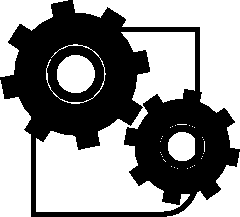
\includegraphics[width=0.75cm]{col11305.imgs/summary_simulation.png} &   \end{array} $ \hspace{2 pt}\raisebox{-5 pt}{} {(section shortcode: P10067 )} \par 
\begin{minipage}{.5\textwidth}      
\label{m37830*id129246}A \textbf{compass} is an instrument which is used to find the direction of a
magnetic
field. A compass consists of a small metal needle which
is magnetised itself and which is free to turn in any direction.
Therefore, when in the presence of a magnetic field,
the needle is able to line up in the same direction as the field.\par 
\end{minipage}
\begin{minipage}{.5\textwidth}      
\begin{figure}[H] % horizontal\label{m37830*id128235}
    \begin{center}
    \begin{pspicture}(0,-1.4)(6.02125,1.4)
\definecolor{color1276b}{rgb}{0.4,0.4,0.4}
\pscircle[linewidth=0.07,dimen=outer](1.4,0.0){1.3}
\rput(1.4098438,1.05){N}
\rput(1.3792187,-1.05){S}
\rput(0.40609375,0.01){W}
\rput(2.4020312,0.01){E}
\pscircle[linewidth=0.07,dimen=outer](1.4,0.0){1.4}
\rput(0.79296875,0.725){\scriptsize NW}
\rput(2.0842187,0.725){\scriptsize NE}
\rput(0.7423437,-0.755){\scriptsize SW}
\rput(2.0735939,-0.755){\scriptsize SE}
\psdiamond[linewidth=0.04,dimen=outer,gangle=-89.052](1.39,-0.00955629)(0.15,0.8504437)
\psline[linewidth=0.04cm](0.76,0.0)(2.14,0.0)
\psdiamond[linewidth=0.04,dimen=outer](1.4,-0.00955629)(0.18,0.9104437)
\pspolygon[linewidth=0.04,fillstyle=solid,fillcolor=color1276b](1.24,-0.0014992657)(1.4,0.80420315)(1.54,-0.0014992657)
\pscircle[linewidth=0.04,dimen=outer,fillstyle=solid,fillcolor=black](1.3844562,-0.0014992657){0.064456195}
\pspolygon[linewidth=0.04,fillstyle=solid](1.4,-0.78)(1.54,-0.02)(1.24,-0.02)
\pscircle[linewidth=0.04,dimen=outer,fillstyle=solid,fillcolor=black](1.3844562,-0.021499265){0.064456195}
\psline[linewidth=0.04cm](1.38,0.32)(3.4,0.8)
\psline[linewidth=0.04cm](1.38,0.0)(3.4,-0.42)
\rput(4.729219,0.84){\small magnetised needle}
\rput(3.798125,-0.42){\small pivot}
\end{pspicture} \end{center}
 \end{figure}
\end{minipage}

      \label{m37830*id127852}
    \setcounter{subfigure}{0}
	\begin{figure}[H] % horizontal\label{m37830*id127855}
    \begin{center}
    \begin{pspicture}(0,-3.4589062)(6.0834374,3.4389062)
\definecolor{color60}{rgb}{0.6,0.6,0.6}
\psframe[fillstyle=solid,fillcolor=red,linewidth=0.04,dimen=outer](3.419,0.9866473)(2.626,-0.996802)
\psbezier[linewidth=0.04,linecolor=color60](3.2359998,0.9866473)(4.0514936,2.029044)(4.28825,-1.807555)(3.249153,-0.9678465)
\psbezier[linewidth=0.04,linecolor=color60](2.7937498,0.9866473)(1.9782562,2.029044)(1.7414999,-1.807555)(2.7805967,-0.9678465)
\psbezier[linewidth=0.04,linecolor=color60](3.1444998,0.9721696)(4.47125,2.5068092)(4.822,-2.2418869)(3.1444998,-0.98232424)
\psbezier[linewidth=0.04,linecolor=color60](2.9004998,0.9866473)(1.5737499,2.5502424)(1.23825,-2.2129314)(2.87,-0.98232424)
\psbezier[linewidth=0.04,linecolor=color60](3.0835,0.9721696)(5.17275,3.4044285)(5.4624996,-3.2408504)(3.0835,-0.98232424)
\psbezier[linewidth=0.04,linecolor=color60](2.9615,0.9866473)(0.87224996,3.4189062)(0.5825,-3.2263727)(2.9615,-0.9678465)
\psbezier[linewidth=0.04,linecolor=color60](3.06825,-0.9678465)(3.1497178,-1.9022263)(4.583618,-2.0971096)(4.8677497,-1.7426693)
\psbezier[linewidth=0.04,linecolor=color60](2.9615,-0.9678465)(2.880032,-1.9022263)(1.5584999,-2.0102432)(1.2535,-1.7206886)
\psbezier[linewidth=0.04,linecolor=color60,arrowsize=0.05291667cm 3.0,arrowlength=1.4,arrowinset=0.25]{->}(2.9919999,0.95769185)(2.910532,1.8920717)(1.589,2.0000885)(1.2839999,1.7105339)
\psbezier[linewidth=0.04,linecolor=color60,arrowsize=0.05291667cm 3.0,arrowlength=1.4,arrowinset=0.25]{->}(3.0835,0.95769185)(3.1649678,1.8920717)(4.5988684,2.0869548)(4.883,1.7325147)
\psbezier[linewidth=0.04,linecolor=color60](3.0224998,-0.98232424)(3.1192176,-1.9311818)(3.61725,-2.0826318)(4.4102497,-2.183976)
\psbezier[linewidth=0.04,linecolor=color60,arrowsize=0.05291667cm 3.0,arrowlength=1.4,arrowinset=0.25]{<-}(3.0072498,-0.9678465)(2.910532,-1.916704)(2.4125,-2.068154)(1.6194999,-2.1694982)
\psbezier[linewidth=0.04,linecolor=color60,arrowsize=0.05291667cm 3.0,arrowlength=1.4,arrowinset=0.25]{->}(3.0072498,0.9721696)(2.910532,1.9210272)(2.4125,2.072477)(1.6194999,2.1738212)
\psbezier[linewidth=0.04,linecolor=color60,arrowsize=0.05291667cm 3.0,arrowlength=1.4,arrowinset=0.25]{->}(3.053,0.9721696)(3.1497178,1.9210272)(3.64775,2.072477)(4.4407496,2.1738212)
\psline[linewidth=0.04cm,linecolor=color60,arrowsize=0.05291667cm 3.0,arrowlength=1.4,arrowinset=0.25]{->}(3.03775,0.9721696)(3.03775,2.5502424)
\psline[linewidth=0.04cm,linecolor=color60,arrowsize=0.05291667cm 2.0,arrowlength=1.4,arrowinset=0.4]{->}(3.0072498,-2.5314415)(3.0072498,-0.9533688)
\psbezier[linewidth=0.04](3.1120791,-0.6608777)(3.0327232,-0.6313349)(2.9742334,-0.6730593)(2.9965632,-0.7232172)(3.0188928,-0.7733751)(3.0925786,-0.7383254)(3.1139057,-0.7960709)(3.1352324,-0.85381633)(3.0442836,-0.88503647)(2.9605973,-0.82630384)
\psline[linewidth=0.04cm](2.94625,0.8997809)(2.94625,0.65365946)
\psline[linewidth=0.04cm](2.94625,0.8997809)(3.1139998,0.6681372)
\psline[linewidth=0.04cm](3.1139998,0.6681372)(3.1139998,0.8853032)
\psbezier[linewidth=0.04,linecolor=color60,arrowsize=0.05291667cm 3.0,arrowlength=1.4,arrowinset=0.25]{<-}(2.809,-1.6482999)(2.51925,-2.0826318)(1.8939999,-2.1115873)(1.6194999,-2.183976)
\psbezier[linewidth=0.04,linecolor=color60,arrowsize=0.05291667cm 3.0,arrowlength=1.4,arrowinset=0.25]{<-}(2.48875,-1.7013849)(2.077,-1.9233768)(1.3907499,-1.8944213)(1.2535,-1.7062109)
\psline[linewidth=0.04cm,linecolor=color60,arrowsize=0.05291667cm 3.0,arrowlength=1.4,arrowinset=0.25]{->}(3.0072498,-2.4590528)(3.0072498,-1.6772554)
\psbezier[linewidth=0.04,linecolor=color60,arrowsize=0.05291667cm 3.0,arrowlength=1.4,arrowinset=0.25]{<-}(3.3579998,-1.749644)(3.4342499,-1.9523323)(4.029,-2.183976)(4.395,-2.1694982)
\psbezier[linewidth=0.04,linecolor=color60,arrowsize=0.05291667cm 3.0,arrowlength=1.4,arrowinset=0.25]{<-}(3.5867498,-1.6917331)(3.846,-1.8944213)(4.6085,-2.0102432)(4.883,-1.749644)
\psbezier[linewidth=0.04,linecolor=color60,arrowsize=0.05291667cm 3.0,arrowlength=1.4,arrowinset=0.25]{->}(3.2359998,0.9866473)(3.7849998,1.6671007)(3.9374998,0.24828297)(3.9374998,-0.070227124)
\psbezier[linewidth=0.04,linecolor=color60,arrowsize=0.05291667cm 3.0,arrowlength=1.4,arrowinset=0.25]{->}(3.15975,0.9721696)(4.029,1.9132222)(4.2425,0.45097122)(4.3034997,-0.055749394)
\psbezier[linewidth=0.04,linecolor=color60,arrowsize=0.05291667cm 3.0,arrowlength=1.4,arrowinset=0.25]{->}(3.0835,0.9866473)(4.395,2.4199429)(4.7609997,0.5667931)(4.7609997,-0.055749394)
\psbezier[linewidth=0.04,linecolor=color60,arrowsize=0.05291667cm 3.0,arrowlength=1.4,arrowinset=0.25]{->}(2.7937498,0.9866473)(2.2294998,1.6381452)(2.0922499,0.2627607)(2.0922499,-0.070227124)
\psbezier[linewidth=0.04,linecolor=color60,arrowsize=0.05291667cm 3.0,arrowlength=1.4,arrowinset=0.25]{->}(2.9004998,0.9866473)(1.9245,2.0145662)(1.772,0.23380524)(1.8024999,-0.070227124)
\psbezier[linewidth=0.04,linecolor=color60,arrowsize=0.05291667cm 3.0,arrowlength=1.4,arrowinset=0.25]{->}(2.94625,1.001125)(1.589,2.4778538)(1.26875,0.45097122)(1.2839999,-0.09918259)
\pscircle[linewidth=0.078,dimen=outer](5.5125,-0.03109375){0.51}
\pspolygon[linewidth=0.04,fillstyle=solid,fillcolor=black](5.443904,-0.00109375)(5.443904,-0.23806344)(5.3425,-0.22316271)(5.5087137,-0.46109375)(5.6425,-0.24462315)(5.571286,-0.2392114)(5.578153,-0.00109375)
\pscircle[linewidth=0.04,linecolor=white,dimen=outer,fillstyle=solid](5.5025,-0.04109375){0.02}
\pscircle[linewidth=0.078,dimen=outer](0.5125,-0.03109375){0.51}
\pspolygon[linewidth=0.04,fillstyle=solid,fillcolor=black](0.44390392,-0.00109375)(0.44390392,-0.23806344)(0.3425,-0.22316271)(0.50871384,-0.46109375)(0.6425,-0.24462315)(0.57128626,-0.2392114)(0.578153,-0.00109375)
\pscircle[linewidth=0.04,linecolor=white,dimen=outer,fillstyle=solid](0.5025,-0.04109375){0.02}
\rput{-79.904144}(6.0744042,3.309316){\pscircle[linewidth=0.078,dimen=outer,fillstyle=solid](5.0125,-1.9710938){0.51}}
\pspolygon[linewidth=0.04,fillstyle=solid,fillcolor=black](5.0300107,-1.898301)(4.7967105,-1.9398407)(4.793605,-1.8373948)(4.5884943,-2.0427432)(4.825065,-2.1365116)(4.8179097,-2.0654519)(5.053544,-2.0304713)
\rput{-79.904144}(6.0568724,3.304571){\pscircle[linewidth=0.04,linecolor=white,dimen=outer,fillstyle=solid](5.0009017,-1.9630015){0.02}}
\rput{-101.33104}(0.30287695,4.786019){\pscircle[linewidth=0.078,dimen=outer,fillstyle=solid](2.1125,2.2689064){0.51}}
\pspolygon[linewidth=0.04,fillstyle=solid,fillcolor=black](2.155393,2.330271)(1.923042,2.37683)(1.9575759,2.4733298)(1.6916254,2.3571038)(1.8775905,2.183394)(1.8968887,2.2521563)(2.129016,2.1986387)
\rput{-101.33104}(0.28195578,4.7924137){\pscircle[linewidth=0.04,linecolor=white,dimen=outer,fillstyle=solid](2.1046598,2.2806761){0.02}}
\rput(3.0170312,-2.8310938){The direction of the compass arrow is the }
\rput(3.0042188,-3.2310936){same as the direction of the magnetic field}
\end{pspicture} 
\end{center}
 \end{figure}       
      \par 
\IFact{      \label{m37830*id127867}Lodestone, a magnetised form of iron-oxide, was found to orientate itself
in a north-south direction if left free to rotate by suspension
on a string or on a float in water. Lodestone was therefore used as
an early navigational compass.}
\begin{minipage}{.5\textwidth}
      \label{m37830*id128225}Compasses are mainly used in navigation to find direction on the earth.
This works because
the Earth  itself has a magnetic field which is similar to that of a bar magnet
(see the picture below). The compass needle aligns with the Earth's magnetic field
direction and points north-south. Once you know where north is, you can
figure out any other direction. A photograph of a compass is shown on the right.\par 
\label{m37830*id128241}Some animals can detect magnetic fields, which
helps them orientate themselves and navigate. Animals which can do this include pigeons, bees, Monarch
butterflies, sea turtles and certain fish.\par 
     
\end{minipage}
\begin{minipage}{.5\textwidth}
\begin{center}
\textbf{A compass}\par
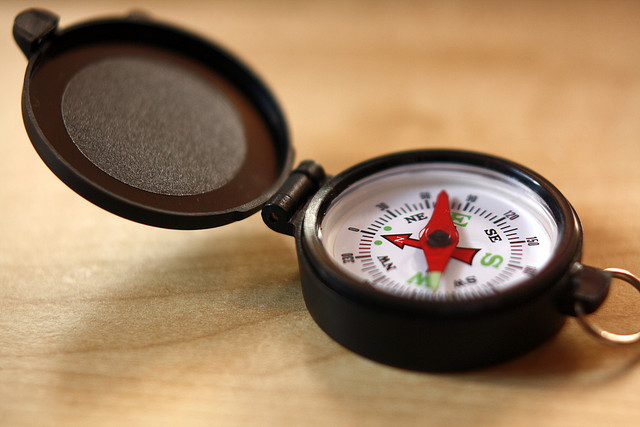
\includegraphics[width=.8\textwidth]{photos/Colin_ZHU.jpg}\par
\textit{A photograph by Colin Zhu}
\end{center}
\end{minipage}
       \label{m37830*uid22}
            \subsection*{The Earth's magnetic field}
            \nopagebreak
        \label{m37830*id128255}In the picture below, you can see a representation of the Earth's magnetic
field which is very similar to the magnetic field of a giant bar magnet like
the one on the right of the picture. The Earth  has two geographic poles which are the points on the Earth's surface
where the line of the Earth's axis of rotation meets the surface. To visualise this you could take any round fruit (lemon, orange etc.) and stick a pencil through the middle so it comes out the other side. Turn the pencil, the pencil is the axis of rotation
and the geographic poles are where the pencil enters and exits the fruit.

The Earth  also has a magnetic field and therefore has a north and a south \textbf{magnetic} pole. If you measure the Earth's
magnetic field carefully you will find that the magnetic poles do not correspond precisely to the geographic poles.

So the Earth  has two sets of north poles
and south poles: \textbf{geographic poles} and \textbf{magnetic poles}.\par 
        \label{m37830*id128272}
    \setcounter{subfigure}{0}
	\begin{figure}[H] % horizontal\label{m37830*id128275}
    \begin{center}
    \scalebox{0.95} % Change this value to rescale the drawing.
{
\begin{pspicture}(0,-3.7089062)(15.38,3.72)
\definecolor{color875}{rgb}{0.4,0.4,0.4}
\rput(4.08,3.59){11.5$^{o}$}
\rput(6.0,3.08){Geographic North pole}
\rput(1.85,3.30){\color{color875}Magnetic 'North' pole}
\psbezier[linewidth=0.04,linecolor=color875,arrowsize=0.05291667cm 2.0,arrowlength=1.4,arrowinset=0.4]{->}(3.74,-1.38)(3.9,-2.10)(4.34,-2.58)(4.98,-2.90)
\psbezier[linewidth=0.04,linecolor=color875,arrowsize=0.05291667cm 2.0,arrowlength=1.4,arrowinset=0.4]{->}(3.58,-1.34)(3.1,-3.26)(1.14,-3.10)(1.02,-3.12)
\psbezier[linewidth=0.04,linecolor=color875,arrowsize=0.05291667cm 2.0,arrowlength=1.4,arrowinset=0.4]{->}(3.54,-1.40)(3.38,-2.12)(2.94,-2.60)(2.3,-2.92)
\psbezier[linewidth=0.04,linecolor=color875,arrowsize=0.05291667cm 2.0,arrowlength=1.4,arrowinset=0.4]{->}(3.54,-1.36)(2.26,-3.04)(0.6,-2.50)(0.48,-2.20)
\psbezier[linewidth=0.04,linecolor=color875,arrowsize=0.05291667cm 2.0,arrowlength=1.4,arrowinset=0.4]{->}(3.52,-1.38)(3.06,-1.96)(2.68,-2.20)(2.06,-2.46)
\psbezier[linewidth=0.04,linecolor=color875,arrowsize=0.05291667cm 3.0,arrowlength=1.4,arrowinset=0.4]{->}(3.41,-1.38)(2.05,-1.72)(1.63,-0.90)(1.59,-0.10)
\psline[linewidth=0.04cm,linecolor=color875,linestyle=dashed,dash=0.16cm 0.16cm](3.62,3.35)(3.62,-3.68)
\psline[linewidth=0.04cm](4.18,3.34)(3.11,-3.48)
\psbezier[linewidth=0.04,linecolor=color875](3.82,1.15)(5.93,2.29)(6.54,-2.14)(3.87,-1.36)
\psbezier[linewidth=0.04,linecolor=color875,arrowsize=0.05291667cm 3.0,arrowlength=1.4,arrowinset=0.4]{->}(3.90,-1.36)(5.20,-1.70)(5.61,-0.88)(5.64,-0.08)
\psbezier[linewidth=0.04,linecolor=color875](3.5,1.13)(1.29,2.27)(0.66,-2.16)(3.44,-1.38)
\psbezier[linewidth=0.04,linecolor=color875](3.7,1.15)(6.84,3.47)(7.28,-3.24)(3.76,-1.36)
\psbezier[linewidth=0.04,linecolor=color875,arrowsize=0.05291667cm 3.0,arrowlength=1.4,arrowinset=0.4]{->}(3.78,-1.38)(5.04,-2.06)(6.1,-1.64)(6.24,-0.068)
\psbezier[linewidth=0.04,linecolor=color875](3.58,1.15)(0.44,3.47)(0.0,-3.24)(3.52,-1.36)
\psbezier[linewidth=0.04,linecolor=color875,arrowsize=0.05291667cm 3.0,arrowlength=1.4,arrowinset=0.4]{->}(3.48,-1.38)(2.22,-2.06)(1.18,-1.64)(1.04,-0.048)
\psbezier[linewidth=0.04,linecolor=color875,arrowsize=0.05291667cm 2.0,arrowlength=1.4,arrowinset=0.4]{<-}(3.68,1.15)(4.16,3.07)(6.12,2.91)(6.24,2.93)
\psbezier[linewidth=0.04,linecolor=color875,arrowsize=0.05291667cm 2.0,arrowlength=1.4,arrowinset=0.4]{<-}(3.58,1.15)(3.1,3.07)(1.14,2.91)(1.02,2.93)
\psbezier[linewidth=0.04,linecolor=color875,arrowsize=0.05291667cm 2.0,arrowlength=1.4,arrowinset=0.4]{->}(3.72,-1.34)(4.2,-3.26)(6.16,-3.10)(6.28,-3.12)
\psbezier[linewidth=0.04,linecolor=color875,arrowsize=0.05291667cm 2.0,arrowlength=1.4,arrowinset=0.4]{<-}(3.76,1.15)(5.0332885,2.83)(6.7,2.29)(6.82,1.99)
\psbezier[linewidth=0.04,linecolor=color875,arrowsize=0.05291667cm 2.0,arrowlength=1.4,arrowinset=0.4]{<-}(3.56,1.15)(2.28,2.83)(0.62,2.29)(0.5,1.99)
\psbezier[linewidth=0.04,linecolor=color875,arrowsize=0.05291667cm 2.0,arrowlength=1.4,arrowinset=0.4]{->}(3.76,-1.36)(5.03,-3.04)(6.7,-2.50)(6.82,-2.20)
\psbezier[linewidth=0.04,linecolor=color875,arrowsize=0.05291667cm 2.0,arrowlength=1.4,arrowinset=0.4]{->}(6.84,2.01)(6.24,2.57)(5.053,2.23)(4.78,2.05)
\psbezier[linewidth=0.04,linecolor=color875,arrowsize=0.05291667cm 2.0,arrowlength=1.4,arrowinset=0.4]{->}(0.48,2.01)(1.08,2.57)(2.26,2.23)(2.54,2.05)
\psbezier[linewidth=0.04,linecolor=color875,arrowsize=0.05291667cm 2.0,arrowlength=1.4,arrowinset=0.4]{->}(6.24,2.93)(5.5,2.95)(4.94,2.75)(4.5,2.45)
\psbezier[linewidth=0.04,linecolor=color875,arrowsize=0.05291667cm 2.0,arrowlength=1.4,arrowinset=0.4]{->}(1.14,2.93)(1.56,2.91)(2.32,2.79)(2.8,2.43)
\psbezier[linewidth=0.04,linecolor=color875,arrowsize=0.05291667cm 2.0,arrowlength=1.4,arrowinset=0.4]{->}(3.78,-1.38)(4.24,-1.96)(4.62,-2.20)(5.24,-2.46)
\rput{-19.00}(0.23,1.16){\pscircle[linewidth=0.04,dimen=outer,fillstyle=solid](3.60,-0.11){1.29}}
\psbezier[linewidth=0.04](3.98,0.27)(3.97,0.31)(3.97,0.31)(3.97,0.32)(3.98,0.33)(3.96,0.37)(3.97,0.36)(3.98,0.35)(3.97,0.34)(3.96,0.34)(3.96,0.35)(4.01,0.36)(3.98,0.36)(3.95,0.36)(3.98,0.47)(3.72,0.45)(3.47,0.43)(3.68,0.56)(3.60,0.57)(3.51,0.58)(3.50,0.57)(3.35,0.55)(3.21,0.53)(3.09,0.52)(2.96,0.37)(2.832,0.2295)(2.731,-0.0794)(2.908,-0.1861)(3.084,-0.292)(3.310,-0.261)(3.358,-0.343)(3.406,-0.426)(3.290,-0.703)(3.383,-0.809)(3.477,-0.914)(3.425,-1.007)(3.469,-1.053)(3.513,-1.099)(3.676,-1.124)(3.738,-1.066)(3.801,-1.008)(3.855,-0.837)(3.958,-0.8094)(4.0619,-0.7816)(4.004,-0.485)(4.127,-0.434)(4.249,-0.383)(4.382,-0.238)(4.426,-0.166)(4.469,-0.0952)(4.290,-0.185)(4.173,-0.1098)(4.055,-0.0342)(3.994,0.232)(3.983,0.274)
\psbezier[linewidth=0.04](3.940,0.38)(3.92,0.18)(4.33,-0.04)(4.28,-0.045)(4.24,-0.046)(4.55,0.012)(4.52,0.17)(4.49,0.33)(4.18,0.074)(4.27,0.27)(4.36,0.47)(4.88,-0.05)(4.81,0.03)(4.74,0.11)(4.8,0.41)(4.6,0.56)(4.51,0.71)(4.24,1.14)(3.85,1.09)(3.47,1.04)(3.89,0.82)(3.58,0.93)(3.27,1.04)(3.07,0.58)(3.28,0.65)(3.48,0.72)(3.72,0.68)(3.76,0.65)(3.80,0.63)(3.95,0.54)(4.08,0.61)(4.20,0.68)(4.15,0.00)(3.97,0.30)
\psbezier[linewidth=0.04](2.35,0.13)(2.53,-0.64)(2.64,-0.19)(2.68,-0.45)(2.72,-0.71)(2.67,-0.57)(2.69,-0.81)(2.71,-1.05)(2.73,-1.08)(2.72,-0.99)(2.71,-0.91)(2.63,-1.11)(2.70,-0.99)
\psarc[linewidth=0.04](3.86,2.91){0.34}{37.87}{135.0}

\psbezier[linewidth=0.04,linecolor=color875,arrowsize=0.05291667cm 2.0,arrowlength=1.4,arrowinset=0.4]{->}(11.82,-1.36)(11.98,-2.08)(12.42,-2.56)(13.06,-2.88)
\psbezier[linewidth=0.04,linecolor=color875,arrowsize=0.05291667cm 2.0,arrowlength=1.4,arrowinset=0.4]{->}(11.66,-1.32)(11.18,-3.24)(9.22,-3.0)(9.1,-3.10)
\psbezier[linewidth=0.04,linecolor=color875,arrowsize=0.05291667cm 2.0,arrowlength=1.4,arrowinset=0.4]{->}(11.62,-1.38)(11.46,-2.10)(11.02,-2.58)(10.38,-2.90)
\psbezier[linewidth=0.04,linecolor=color875,arrowsize=0.05291667cm 2.0,arrowlength=1.4,arrowinset=0.4]{->}(11.62,-1.34)(10.34,-3.02)(8.68,-2.48)(8.56,-2.18)
\psbezier[linewidth=0.04,linecolor=color875,arrowsize=0.05291667cm 2.0,arrowlength=1.4,arrowinset=0.4]{->}(11.6,-1.36)(11.14,-1.94)(10.76,-2.18)(10.14,-2.44)
\psbezier[linewidth=0.04,linecolor=color875,arrowsize=0.05291667cm 3.0,arrowlength=1.4,arrowinset=0.4]{->}(11.49,-1.36)(10.13,-1.70)(9.71,-0.88)(9.67,-0.08)
\psline[linewidth=0.04cm,linecolor=color875,linestyle=dashed,dash=0.16cm 0.16cm](11.7,3.3710938)(11.7,-3.6689062)
\psbezier[linewidth=0.04,linecolor=color875](11.9,1.17)(14.01,2.31)(14.62,-2.12)(11.9,-1.34)
\psbezier[linewidth=0.04,linecolor=color875,arrowsize=0.05291667cm 3.0,arrowlength=1.4,arrowinset=0.4]{->}(11.98,-1.34)(13.28,-1.68)(13.69,-0.86)(13.72,-0.06)
\psbezier[linewidth=0.04,linecolor=color875](11.58,1.15)(9.37,2.29)(8.74,-2.14)(11.52,-1.36)
\psbezier[linewidth=0.04,linecolor=color875](11.78,1.17)(14.92,3.49)(15.36,-3.22)(11.84,-1.34)
\psbezier[linewidth=0.04,linecolor=color875,arrowsize=0.05291667cm 3.0,arrowlength=1.4,arrowinset=0.4]{->}(11.86,-1.36)(13.12,-2.04)(14.18,-1.62)(14.32,-0.04)
\psbezier[linewidth=0.04,linecolor=color875](11.66,1.17)(8.52,3.49)(8.08,-3.22)(11.6,-1.34)
\psbezier[linewidth=0.04,linecolor=color875,arrowsize=0.05291667cm 3.0,arrowlength=1.4,arrowinset=0.4]{->}(11.56,-1.36)(10.3,-2.04)(9.26,-1.62)(9.12,-0.02)
\psbezier[linewidth=0.04,linecolor=color875,arrowsize=0.05291667cm 2.0,arrowlength=1.4,arrowinset=0.4]{<-}(11.76,1.17)(12.24,3.09)(14.2,2.93)(14.32,2.95)
\psbezier[linewidth=0.04,linecolor=color875,arrowsize=0.05291667cm 2.0,arrowlength=1.4,arrowinset=0.4]{<-}(11.66,1.17)(11.18,3.09)(9.22,2.93)(9.1,2.95)
\psbezier[linewidth=0.04,linecolor=color875,arrowsize=0.05291667cm 2.0,arrowlength=1.4,arrowinset=0.4]{->}(11.8,-1.32)(12.28,-3.24)(14.24,-3.08)(14.36,-3.10)
\psbezier[linewidth=0.04,linecolor=color875,arrowsize=0.05291667cm 2.0,arrowlength=1.4,arrowinset=0.4]{<-}(11.84,1.17)(13.11,2.85)(14.78,2.31)(14.9,2.01)
\psbezier[linewidth=0.04,linecolor=color875,arrowsize=0.05291667cm 2.0,arrowlength=1.4,arrowinset=0.4]{<-}(11.64,1.17)(10.36,2.85)(8.7,2.31)(8.58,2.01)
\psbezier[linewidth=0.04,linecolor=color875,arrowsize=0.05291667cm 2.0,arrowlength=1.4,arrowinset=0.4]{->}(11.84,-1.34)(13.11,-3.02)(14.78,-2.48)(14.9,-2.18)
\psbezier[linewidth=0.04,linecolor=color875,arrowsize=0.05291667cm 2.0,arrowlength=1.4,arrowinset=0.4]{->}(14.92,2.03)(14.32,2.59)(13.13,2.25)(12.86,2.07)
\psbezier[linewidth=0.04,linecolor=color875,arrowsize=0.05291667cm 2.0,arrowlength=1.4,arrowinset=0.4]{->}(8.56,2.03)(9.16,2.59)(10.34,2.25)(10.62,2.07)
\psbezier[linewidth=0.04,linecolor=color875,arrowsize=0.05291667cm 2.0,arrowlength=1.4,arrowinset=0.4]{->}(14.32,2.95)(13.58,2.97)(13.02,2.77)(12.58,2.47)
\psbezier[linewidth=0.04,linecolor=color875,arrowsize=0.05291667cm 2.0,arrowlength=1.4,arrowinset=0.4]{->}(9.22,2.95)(9.64,2.93)(10.4,2.81)(10.88,2.45)
\psbezier[linewidth=0.04,linecolor=color875,arrowsize=0.05291667cm 2.0,arrowlength=1.4,arrowinset=0.4]{->}(11.86,-1.36)(12.32,-1.94)(12.7,-2.18)(13.32,-2.44)
\psframe[fillstyle=solid,fillcolor=red,linewidth=0.04,dimen=outer,fillstyle=solid](12.2,1.23)(11.22,-1.36)
\rput(11.65,0.96){S}
\rput(11.72,-1.09){N}
\end{pspicture} 
}\end{center}
 \end{figure}       
        \par 
        \label{m37830*id129590}The Earth's magnetic field is thought to be caused by flowing liquid metals
in the outer core which causes electric currents and a magnetic field. From the picture
you can see that the direction of magnetic north and true north are not
identical. The \textbf{geographic north pole}, which is the point through which
the Earth's rotation axis goes, is about 11,5$^\text{o}$ away from the direction of
the \textbf{magnetic north pole} (which is where a compass will point). However,
the magnetic poles shift slightly all the time.\par 
        \label{m37830*id129612}Another interesting thing to note is that if we think of the Earth  as a big
bar magnet, and we know that magnetic field lines always point
\textsl{from north to south}, then the compass tells us that what we call the
\textsl{magnetic north pole} is actually the \textsl{south pole} of the bar magnet!\par 
\IFact{  \label{m37830*id129640}The direction of the Earth's magnetic field flips direction about once every
200~000 years! You can picture this as a bar magnet whose north and south pole
periodically switch sides. The reason for this is still not fully understood.\par 
	}
\label{m37830*fs-id1166240854705}
            \subsection{Phenomena related to the Earth's magnetic field }
            \nopagebreak
\label{m37830*fs-id7505799}
            \subsection{The importance of the magnetic field to life on Earth }
            \nopagebreak
\label{m37830*fs-id1166211137674}The Earth's magnetic field is very important for humans and other animals on Earth because it protects us from being bombarded (hit) by high energy charged particles which are emitted by the Sun. The stream of charged particles (mainly positively charged protons and negatively charged electrons) coming from the sun is called the solar wind. When these particles come close to the Earth, they become trapped by the Earth's magnetic field and cannot shower down to the surface where they can harm living organisms. 
Astronauts in space are at risk of being irradiated by the solar wind because they are outside the zones where the charged particles are trapped. 
\par  
\label{m37830*fs-id1166236522828}
\begin{minipage}{.5\textwidth}
 \begin{center}
  \textbf{Visualisation of the magnetosphere}\par
  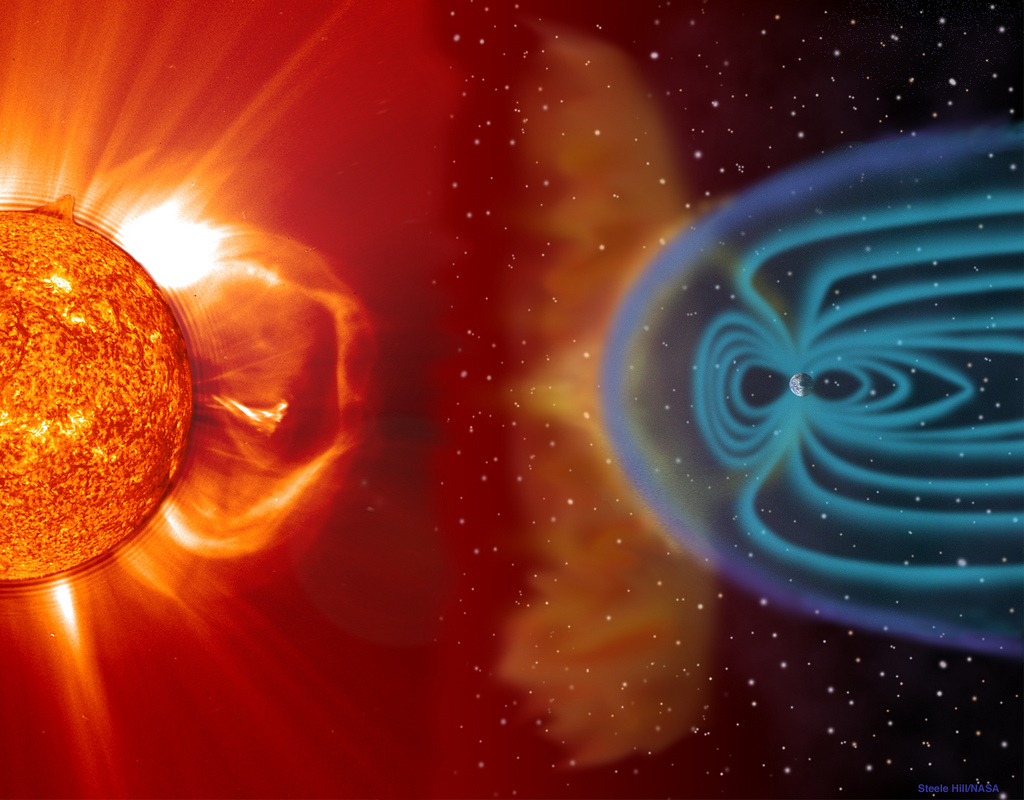
\includegraphics[width=.8\textwidth]{photos/magnetosphere.jpg}\par
  \textit{Graphic by NASA Goddard Photo and Video on Flickr}
 \end{center}
\end{minipage}
\begin{minipage}{.5\textwidth}

The region above Earth's atmosphere in which charged particles are affected by Earth's magnetic field is called the magnetosphere. 
Relatively often, in addition to the usual solar wind, the Sun may eject a large bubble of material (protons and electrons) with its own magnetic field from its outer atmosphere. Sometimes these bubbles travel towards the Earth where their magnetic fields can join with Earth's magnetic field. When this happens a huge amount of energy is released into the Earth's magnetosphere, causing a geomagnetic storm. These storms cause rapid changes in the Earth's magnetosphere which in turn may affect electric and magnetic systems on the Earth such as power grids, cellphone networks, and other electronic systems.
\end{minipage}
\par 
\label{m37830*fs-id1166218597625}
            \subsection{Aurorae (pronounced Or-roar-ee) }
            \nopagebreak
\label{m37830*fs-id1166211416999}
Another effect caused by the Earth's magnetic field is the spectacular Northern and Southern Lights, which are also called the Aurora Borealis and the Aurora Australis respectively.\par
\begin{minipage}{.6\textwidth}
 When charged particles from the solar wind reach the Earth's magnetosphere, they spiral along the magnetic field lines towards the North and South poles. If they collide with particles in the Earth's atmosphere, they can cause red or green lights which stretch across a large part of the sky and which is called the aurora. 
\begin{center}
  \textbf{Aurora borealis photographed in Alaska}\par
  \includegraphics[width=.8\textwidth]{photos/aurora_borealis_Trodel.jpg}\par
  \textit{Photograph by Trodel on Flickr}
 \end{center}
\end{minipage}
\begin{minipage}{.4\textwidth}
 \begin{center}
  \textbf{Aurora australis photographed from space}\par
  \includegraphics[width=.9\textwidth]{photos/aurora_australis_seishin17.jpg}\par
  \textit{Photograph by seishin17 on Flickr}
 \end{center}
\end{minipage}


As this only happens close to the North and South poles, we cannot see the aurorae from South Africa. However, people living in the high Northern latitudes in Canada, Sweden, and Finland, for example, often see the Northern lights.  
\par 
\label{m37830*eip-356}This simulation shows you the Earth's magnetic field and a compass.$ \begin{array}{cccccccccccc}   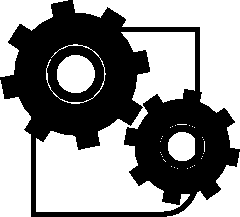
\includegraphics[width=0.5cm]{col11305.imgs/summary_simulation.png} &   \end{array} $ \hspace{1 pt}\raisebox{-5 pt}{} {(Simulation: lb9) } \par 
\section{ Summary}
            \nopagebreak
%            \label{m37830*cid6} $ \hspace{-5pt}\begin{array}{cccccccccccc}   
\includegraphics[width=0.75cm]{col11305.imgs/summary_video.png} &   \end{array} $ \hspace{2 pt}\raisebox{-5 pt}{} {(section shortcode: P10068 )} \par 
      \label{m37830*id129673}\begin{enumerate}[noitemsep, label=\textbf{\arabic*}. ] 
            \label{m37830*uid23}\item Magnets have two poles - North and South.
\label{m37830*uid24}\item Some substances can be easily magnetised.
\label{m37830*uid25}\item Like poles repel each other and unlike poles attract each other.
\label{m37830*uid26}\item The Earth also has a magnetic field.
\label{m37830*uid27}\item A compass can be used to find the magnetic north pole and help us find our direction.
\end{enumerate}
        \label{m37830*eip-568}This video provides a summary of the work covered in this chapter.
    \setcounter{subfigure}{0}
	\begin{figure}[H] % horizontal\label{m37830*magnets-1}
    \textnormal{Khan academy video on magnets} \nopagebreak
  \label{m37830*yt-media1}\label{m37830*yt-video1}
            \raisebox{-5 pt}{ 
\includegraphics[width=0.5cm]{col11305.imgs/summary_www.png}} { (Video:  P10069 )}
 \end{figure}       \par 
\begin{eocexercises}{ End of chapter exercises}
            \nopagebreak
%            \label{m37830*cid7} $ \hspace{-5pt}\begin{array}{cccccccccccc}   \end{array} $ \hspace{2 pt}\raisebox{-0.2em}{
\includegraphics[height=1em]{../icons/www.eps}} {(section shortcode: P10070 )} \par 
      \label{m37830*id129746}\begin{enumerate}[noitemsep, label=\textbf{\arabic*}. ] 
            \label{m37830*uid28}\item Describe what is meant by the term \textsl{magnetic field}.\newline
\label{m37830*uid29}\item Use words and pictures to explain why permanent magnets have a magnetic field around them. Refer to \textsl{domains} in your explanation.\newline
\label{m37830*uid30}\item What is a magnet?\newline
\label{m37830*uid31}\item What happens to the poles of a magnet if it is cut into pieces?\newline
\label{m37830*uid32}\item What happens when like magnetic poles are brought close together?\newline
\label{m37830*uid33}\item What happens when unlike magnetic poles are brought close together?\newline
\label{m37830*uid34}\item Draw the shape of the magnetic field around a bar magnet.\newline
\label{m37830*uid35}\item Explain how a compass indicates the direction of a magnetic field.\newline
\label{m37830*uid36}\item Compare the magnetic field of the Earth to the magnetic field of a bar magnet using words and diagrams.\newline
\label{m37830*uid37}\item Explain the difference between the geographical north pole and the magnetic north pole of the Earth.\newline
\label{m37830*uid38}\item Give examples of phenomena that are affected by Earth's magnetic field.\newline
\label{m37830*uid39}\item Draw a diagram showing the magnetic field around the Earth.\newline
\end{enumerate}
  \label{m37830**end}
\par \raisebox{-0.2em}{
\includegraphics[height=1em]{../icons/www.eps}} Find the answers with the shortcodes:
 \par \begin{tabular}[h]{cccccc}
 (1.) llS  &  (2.) lia  &  (3.) lix  &  (4.) lic  &  (5.) liO  &  (6.) li3  &  (7.) lii  &  (8.) llu  &  (9.) lil  &  (10.) llh  &  (11.) llJ  &  (12.) llt  & \end{tabular}
\end{eocexercises}